%&../preamble

\def\npart {IA}
\def\nterm {Michaelmas}
\def\nyear {2021}
\def\nlecturer {R.\ Camina}
\def\ncourse {Groups}
\def\nauthor{Author}

\def\encodingdefault{TU}\normalfont
\ifnum 0\ifxetex 1\fi\ifluatex 1\fi=0 % if pdftex
  \usepackage[T1]{fontenc}
  \usepackage[utf8]{inputenc}
  \usepackage{textcomp} % provide euro and other symbols
\else % if luatex or xetex
  % \usepackage{unicode-math}
  % \defaultfontfeatures{Scale=MatchLowercase}
  % \defaultfontfeatures[\rmfamily]{Ligatures=TeX,Scale=1}
  % \DeclareMathAlphabet{\mathcal}{OMS}{cmsy}{m}{n}
  % \let\mathbb\relax % remove the definition by unicode-math
  % \DeclareMathAlphabet{\mathbb}{U}{msb}{m}{n}
\fi

\usetikzlibrary{external}
\tikzset{external/system call={xelatex -fmt=../preamble.fmt \tikzexternalcheckshellescape -halt-on-error -interaction=batchmode -jobname "\image" "\texsource"}} % path is relative to file that includes preamble
\tikzexternalize

\providetoggle{DontSetTitleAuthorDate}

\nottoggle{DontSetTitleAuthorDate}{
  \hypersetup{
    pdftitle={Part \npart\ - \ncourse},
    pdfsubject={Cambridge Maths Notes: Part \npart\ - \ncourse},
    pdfkeywords={Cambridge Mathematics Maths Math \npart\ \nterm\ \nyear\ \ncourse}
  }

  \author{Based on lectures by \nlecturer}
  \date{\nterm\ \nyear}
  \title{Part \npart\ --- \ncourse}
}{}

\tikzsetexternalprefix{figtemp/}

% \includeonly{08-mobius.tex}

\begin{document}
\maketitle

\section*{Syllabus}

{\small
  \noindent\textbf{Examples of groups}\\
  Axioms for groups. Examples from geometry: symmetry groups of regular polygons, cube, tetrahedron. Permutations on a set; the symmetric group. Subgroups and homomorphisms. Symmetry groups as subgroups of general permutation groups. The M\"obius group; cross-ratios, preservation of circles, the point at infinity. Conjugation. Fixed points of M\"obius maps and iteration.\hspace*{\fill} [4]

  \vspace{10pt}
  \noindent\textbf{Lagrange's theorem}\\
  Cosets. Lagrange's theorem. Groups of small order (up to order 8). Quaternions. Fermat-Euler theorem from the group-theoretic point of view.\hspace*{\fill} [5]

  \vspace{10pt}
  \noindent\textbf{Group actions}\\
  Group actions; orbits and stabilizers. Orbit-stabilizer theorem. Cayley's theorem (every group is isomorphic to a subgroup of a permutation group). Conjugacy classes. Cauchy's theorem.\hspace*{\fill} [4]

  \vspace{10pt}
  \noindent\textbf{Quotient groups}\\
  Normal subgroups, quotient groups and the isomorphism theorem.\hspace*{\fill} [4]

  \vspace{10pt}
  \noindent
  \textbf{Matrix groups}\\
  The general and special linear groups; relation with the M\"obius group. The orthogonal and special orthogonal groups. Proof (in $\mathbb{R}^3$) that every element of the orthogonal group is the product of reflections and every rotation in $\mathbb{R}^3$ has an axis. Basis change as an example of conjugation.\hspace*{\fill} [3]

  \vspace{10pt}
  \noindent\textbf{Permutations}\\
  Permutations, cycles and transpositions. The sign of a permutation. Conjugacy in $S_n$ and in $A_n$. Simple groups; simplicity of $A_5$.\hspace*{\fill} [4]}

\newpage
\tableofcontents

\hypertarget{Introduction}{%
\section*{Introduction}\label{Introduction}}
\addcontentsline{toc}{section}{Introduction}

Dr Rachel Camina

Recommended books: Algebra \& Geometry, Alan Beardon.

Notation: \Lightning - contradiction

\newpage

\section{Groups and homomorphisms}

\hypertarget{motivation}{%
\subsection{Motivation}\label{motivation}}

Groups are the abstractions of symmetries, a unified way to investigate symmetries.

\hypertarget{basic-definitions-and-examples}{%
\subsection{Basic Definitions and Examples}\label{basic-definitions-and-examples}}

\begin{definition}[binary operation]
  A binary operation,*, on a set \(X\) is a way of combining two elements of \(X\) to unambiguously give another element of \(X\),
i.e.~\(*: X \times X \to X\).
\end{definition} 

\begin{definition}[Group]

If \(G\) is a set and \(*\) is a binary operation on \(G\) then \((G, *)\) is a \emph{group} if the following four axioms hold:

\begin{enumerate}
\def\labelenumi{\arabic{enumi}.}
\item
  \(x, y \in G \implies x * y \in G\) \hfill~{(closure)}
\item
  \(\exists\) an element \(e \in G \text{ satisfying } x * e = x = e * x\) \hfill~{(existence of an identity)}
\item
  for every \(x \in G\) there is a \(y \in G\) s.t. \(x * y = e = y * x\) \hfill~{(existence of inverses)}
\item
  for every \(x, y, z \in G\), \(x * (y * z) = (x * y) * z\) \hfill~{(the associative law)}
\end{enumerate}

\end{definition}

\begin{remark}
\(e\) is called the identity of \(G\) - see \Cref{lem:one} for why it is unique.
We will show in \Cref{lem:one} that inverses are unique and we will write \(x^{-1}\) for the inverse of \(x\).
\end{remark}

\begin{example}
\((\mathbb{Z}, +)\), \(e = 0\), \(x^{-1} = -x\)
\end{example}

\begin{example}
\((\mathbb{Q}, +)\), \((\mathbb{R}, +)\)
\end{example}

\begin{example}
\((\mathbb{Q} \setminus \{ 0 \}, *)\)
\end{example}

\textbf{Non Example 1.1} \((\mathbb{Z}, -)\) - associativity fails

\textbf{Non Example 1.2} \((\mathbb{Z}, *)\) - no inverses

\textbf{Non Example 1.3} \((\mathbb{Q}, *)\) - \(0^{-1}\) does not exist

These have all had an infinite number of elements, so onto some finite groups.

\begin{example}[The trivial group]
\((e, *)\)
\end{example}

\begin{example}
\((\{\pm 1\}, \times)\). A nice way to look at a group is to look at a multiplication table.

\begin{align*}
    \begin{array}{c|cc}
        \times & 1 & -1 \\
        \hline
        1 & 1 & -1 \\
        -1 & -1 & 1 
    \end{array} 
\end{align*}

We can see \(e = 1\) and \((-1)^{-1} = -1\)
\end{example}

\begin{example}
\((\{0, 1, 2\}, +_3)\). \(+_3\) is addition modulo 3.

\begin{align*}
    \begin{array}{c|ccc}
        +_3 & 0 & 1 & 2 \\
        \hline
        0 & 0 & 1 & 2\\
        1 & 1 & 2 & 0 \\
        2 & 2 & 0 & 1
    \end{array} 
\end{align*}

We can see \(e = 0\) and \(1^{-1} = 2\)
\end{example}

\begin{example}
\protect\hypertarget{exm:nine}{}\label{exm:nine}\((\{e, a, b, c\}, *)\)

\begin{align*}
    \begin{array}{c|cccc}
        * & e & a & b & c \\
        \hline
        e & e & a & b & c \\
        a & a & e & c & b \\
        b & b & c & e & a \\
        c & c & b & a & e
    \end{array} 
\end{align*}

You may notice that in any row no element is repeated, this is due to the cancellation law, \Cref{rem:cancellation-law}.
\end{example}

\begin{example}
\protect\hypertarget{exm:triangle}{}\label{exm:triangle}
Rotations and reflections of an equilateral triangle.

{\centering
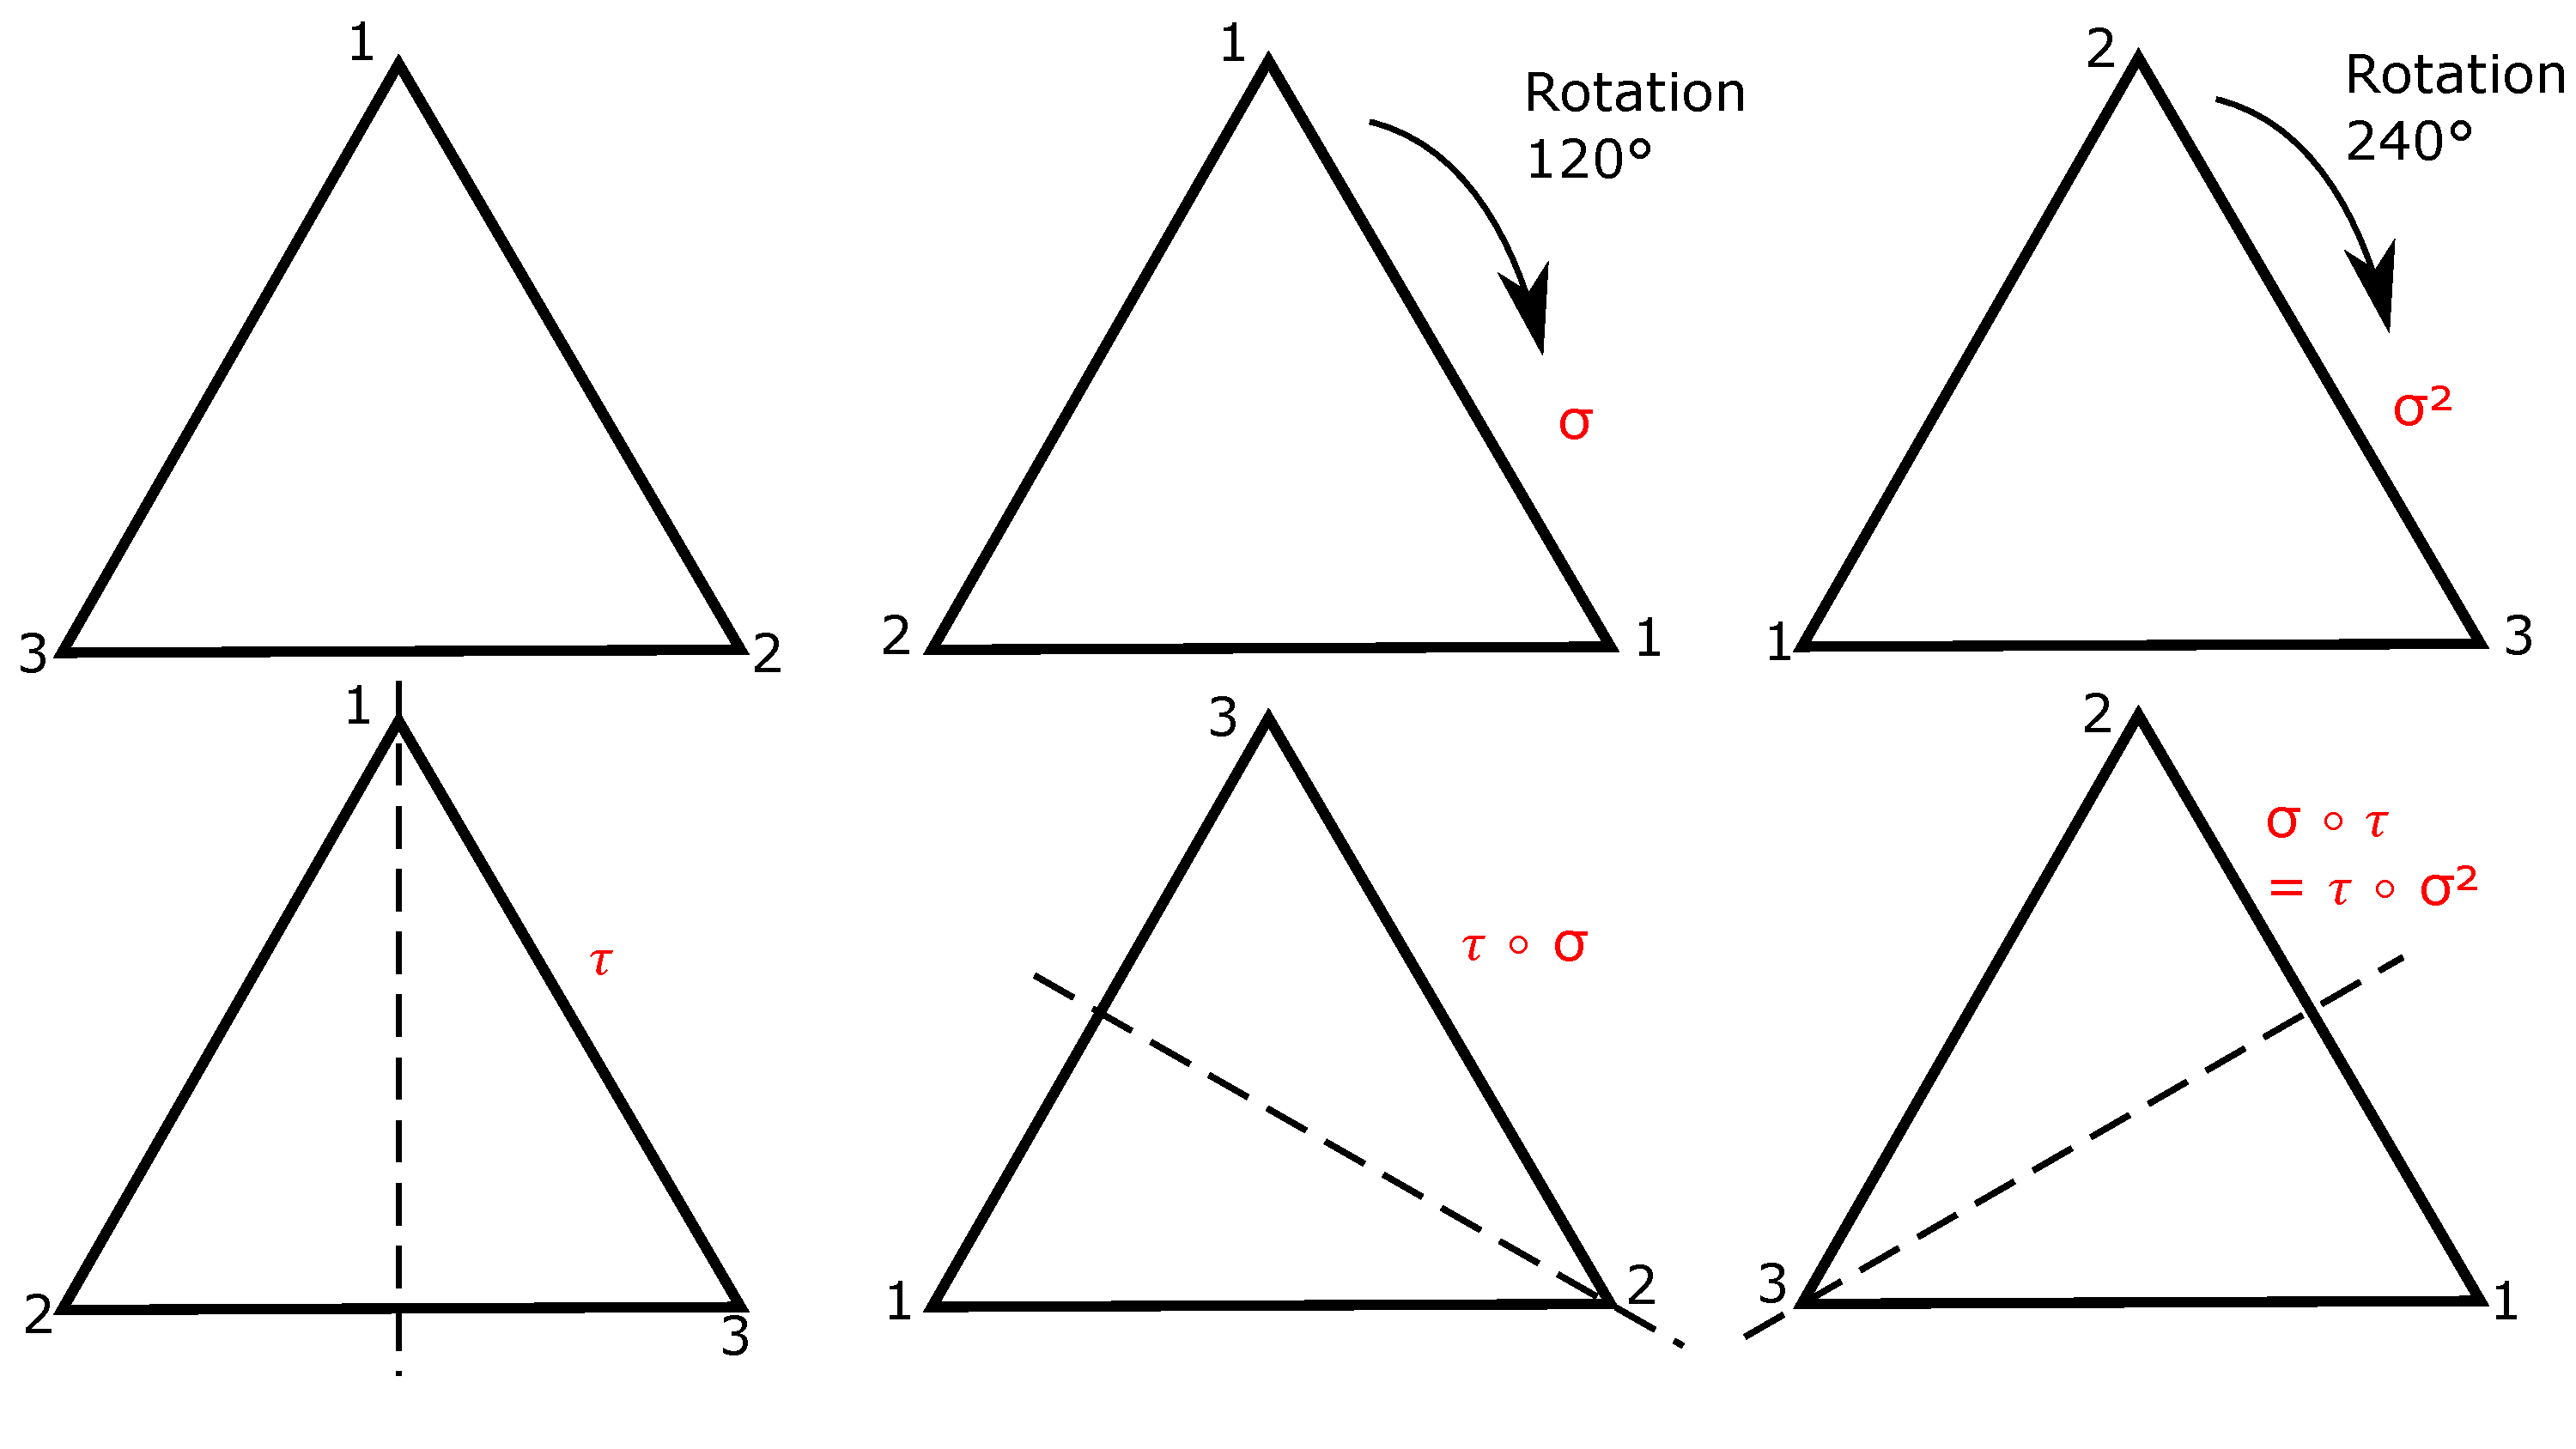
\includegraphics[height=10cm]{01-triangle.pdf}}

operation \(\circ =\) do right transformation then left transformation

\textbf{Claim}: This defines a group with 6 elements
\end{example}

\begin{example}
\begin{align*}
    M_2(\mathbb{R}) &= \{ 2 \times 2 \text{ matrices with entries in } \mathbb{R} \} \\
    &= \left[ \begin{pmatrix} a & b \\ c & d \end{pmatrix} : a, b, c, d \in \mathbb{R} \right] \\
    \intertext{under addition}
    \begin{pmatrix}
    a & b \\
    c & d
    \end{pmatrix} + 
    \begin{pmatrix}
    \alpha & \beta \\
    \gamma & \delta
    \end{pmatrix} &=
    \begin{pmatrix}
    a + \alpha & b + \beta \\
    c + \gamma & d + \delta
    \end{pmatrix}
\end{align*}
\end{example}

A more interesting example is

\begin{example}
\protect\hypertarget{exm:glg}{}\label{exm:glg}\begin{align*}
    GL_2 (\mathbb{R}) &= \{ \text{invertible $2 \times 2$ matrices with entries in } \mathbb{R} \}. \\
    A &= \begin{pmatrix}
    a & b \\
    c & d
    \end{pmatrix},\ \det A = ad - bc \neq 0  \\
    A^{-1} &= \frac{1}{\det A} \begin{pmatrix}
    d & -b \\
    -c & -a
    \end{pmatrix}
\end{align*}

Under multiplication this is a group. \(GL\) stands for general linear group.
\end{example}

\begin{lemma}
\protect\hypertarget{lem:one}{}\label{lem:one}

Let \((G, *)\) be a group.

\begin{enumerate}
\def\labelenumi{\roman{enumi}.}
\item
  The identity element is unique.
\item
  Inverses are unique.
\end{enumerate}

\end{lemma}

\begin{proof}
\mbox{}
\begin{enumerate}
  \def\labelenumi{\roman{enumi}.}
  \item
  Suppose \(e\) and \(\hat{e}\) are both identities, so
  \begin{align*}
      a * e &= a = e * a,\ \ a * \hat{e} = a = \hat{e} * a \hspace{0.4cm }\forall a \in G. \\
      \intertext{In particular}
      e &= e * \hat{e} = \hat{e}.
  \end{align*}
  \item
  Suppose both \(y\) and \(z\) are inverses for \(x\), so
  \begin{align*}
      x * y &= e = y * x,\ \ x * z = e = z * x \\
      \text{Then, } y &= y * e \\
      &= y * (x * z) \\
      &= (y * x) * z \hspace{2cm} \text{(associative law)} \\
      &= e * z \\
      &= z.
  \end{align*}
  \end{enumerate}
\end{proof}

\begin{remark}
Associativity means we don't need brackets, \(x * y * z\) is unambiguous.
Furthermore, by induction, \(x_1 * x_2 * \ldots * x_n\) is unambiguous.

We know the statement is true for the case \(n = 3\).
\begin{align*}
    x_1 * (x_2 * \ldots * x_n) &= (x_1 * x_2) * (x_3 * \ldots * x_n) \\
    &= (x_1 * x_2 * x_3) * (x_4 * \ldots * x_n) \\
    &= \ldots \\
    &= (x_1 * x_2 * \ldots * x_{n-1}) * x_n
\end{align*}
\end{remark}

\begin{remark}
We often omit `\(*\)' and write \(x y\) for \(x * y\) and \(G\) for \((G, *)\).
\end{remark}

\begin{remark}
\((xy)^{-1} = y^{-1} x^{-1}\). Since it works:
\begin{align*}
    (xy)y^{-1}x^{-1} &= x(y y^{-1})x^{-1} \\
    &= x e x^{-1} \\
    &= x x^{-1} \\
    &= e
\end{align*}
\end{remark}
Note, inverses are unique

\begin{remark}
\((x^{-1})^{-1} = x\)
\end{remark}

\begin{remark} \label{rem:cancellation-law}
\begin{align*} 
    && x, y, z \in G &\text{ and } xy = xz \\
    &\implies & x^{-1} x y &= x^{-1} x z \\
    &\implies & y &= z \hspace{3cm} \text{(cancellation law)}
\end{align*}
\end{remark}

%Lecture 2

\begin{definition}[Abelian group]
A group \(G\) is \emph{abelian} (or commutative) if \(xy = yx\) for all \(x, y \in G\).
\end{definition}

Note all our examples above are abelian except \ref{exm:triangle} and \ref{exm:glg}.

\begin{definition}[Order of group]
Let \(G\) be a group. If the number of elements in the set \(G\) is finite, then \(G\) is called a \emph{finite group}. Otherwise, \(G\) is called an \emph{infinite group}. If \(G\) is a finite group denote the number of elements in the set \(G\) by \(|G|\) and call this the \emph{order} of \(G\).
\end{definition}

\begin{definition}[Subgroup]
Let \((G, *)\) be a group and \(H\) a subset of \(G\) (\(H \subseteq G\) i.e.~\(h \in H \implies h \in G\)). Then \((H, *)\) is a \emph{subgroup} of \((G, *)\) if \((H, *)\) is a group (with same operation) i.e.~if

\begin{enumerate}
\def\labelenumi{\alph{enumi})}
\item
  \(h, k \in H \implies h * k \in H\)
\item
  \(e_G \in H\)
\item
  \(h \in H \implies h^{-1} \in H\)
\end{enumerate}

(Note associativity is inherited)

i.e restricting operation to \(H\) still gives a group. We write \(H \leq G\).
\end{definition}

\begin{example}
\begin{align*}
    (\mathbb{Z}, +) \leq (\mathbb{Q}, +) \leq (\mathbb{R}, +)
\end{align*}
\end{example}

\begin{example}
\begin{align*}
    (\{\pm 1\}, \times) \leq (\mathbb{Q} \setminus \{ 0 \}, \times) 
\end{align*}
\end{example}

\begin{example}
In \Cref{exm:triangle} if we just take the rotations we get a subgroup, \(\{ 1, \sigma, \sigma^2 \}\) is a subgroup.
\end{example}

\begin{example}
\protect\hypertarget{exm:sltwo}{}\label{exm:sltwo}
In \Cref{exm:glg}, we can take the matrices with determinant 1 which is \(\mathrm{SL}_2(\mathbb{R})\) (\(\mathrm{SL}\) stands for the special linear group).
\begin{align*}
  \mathrm{SL}_2(\mathbb{R}) &= \{ A \in GL_2(\mathbb{R}) : \det A = 1 \} \\
    &\leq GL_2(\mathbb{R})
\end{align*}
\end{example}

We always have identity and whole thing as subgroups.

\begin{example}
If \(G\) is a group then \(\{ e \} \leq G\) is the trivial subgroup.
\end{example}

\begin{example}
If \(G\) is a group then \(G \leq G\) is the improper subgroup.
\end{example}

\begin{proposition}
\protect\hypertarget{prp:nZ}{}\label{prp:nZ}Subgroups of \(\mathbb{Z}\) are exactly \(n \mathbb{Z} = {nk : k \in \mathbb{Z}}\) where \(n \in \mathbb{Z}_{\geq 0}\) (under addition).
\end{proposition}

\begin{proof}
First note \(n \mathbb{Z}\) is a subgroup of \(\mathbb{Z}\).

\begin{enumerate}
\def\labelenumi{\alph{enumi}.}
\item
  If \(a, b \in n \mathbb{Z}\) then \(a = na'\) and \(b = nb'\) for some \(a', b' \in \mathbb{Z}\).
  Then \(a + b = na' + nb' = n (a' + b') \in n \mathbb{Z}\)
\item
  \(0 \in n \mathbb{Z}\).
\item
  If we have \(a = na' \in n \mathbb{Z}\) then \(a^{-1} = -a = n(-a') \in n \mathbb{Z}\).
\end{enumerate}

Conversely assume \(H \leq \mathbb{Z}\).

If \(H = \{ 0 \} = 0 \mathbb{Z}\).

Otherwise choose \(0 < n \in H\) with \(n\) minimal (smallest positive element of \(H\)).
Then \(n \mathbb{Z} \in H\) by closure and inverses. We show \(H = n \mathbb{Z}\). Suppose \(\exists \; h \in H \setminus n \mathbb{Z}\), then we can write \(h = nk + h'\) with \(h' \in \{ 1, 2, \ldots, n -1 \}\). But \(h' = h - nk \in H\), contradicting minimality of \(n\). Thus \(H = n \mathbb{Z}\).
\end{proof}

\begin{aside}{Aside: Functions}
We need the notion of functions.
\begin{definition}[Function]
  \(f\) is a \emph{function} between sets \(A\) and \(B\) if it assigns each element of \(A\) a unique element of \(B\).
\begin{align*}
    f: A &\to B \\
    a &\mapsto f(a)
\end{align*}
\end{definition} 

\begin{example}
  \begin{align*}
    \text{eg: }\ f: \mathbb{Z} &\to \mathbb{Z} & g: \mathbb{Z} &\to \mathbb{Z} \\
    x &\mapsto x + 1 & x &\mapsto 2x.
  \end{align*}
\end{example} 

\begin{definition}[Composition of functions]
  Suppose \(g: A \to B\) and \(f: B \to C\), define
  \begin{align*}
    f \circ g: A &\to C \\
    a &\mapsto (f \circ g)(a) = f(g(a))
  \end{align*} 
\end{definition} 

\begin{example}
  \begin{align*}
    (f \circ g)(x) &= 2x + 1 \\
    (g \circ f)(x) &= 2x + 2.
  \end{align*} 
\end{example} 

Suppose \(f_1: A \to B\) and \(f_2: A \to B\) then \(f_1 = f_2\) if \(f_1(a) = f_2(a) \quad \forall \; a \in A\).

\begin{definition}[Bijective functions]
  \(f: A \to B\) is a \emph{bijection} if it defines a paring between elements of \(A\) and elements of \(B\). That is given \(b \in B \ \exists\) unique \(a \in A\) s.t. \(f(a) = b\).
\end{definition} 

\begin{example}
  \begin{align*}
    f: \mathbb{Z} &\to \mathbb{Z} \\
    x &\mapsto x + 1
  \end{align*}
\end{example} 

\begin{definition}[Inverse function]
  If we have a bijection we can define
  \begin{align*}
      f^{-1}: B &\to A &&\\
      b &\mapsto a \text{ where } f(a) = b. &&\\
      \text{Then } f \circ f^{-1} &= id_B & f^{-1} \circ f &= id_A \\
      id_B(b) &= b
  \end{align*}
\end{definition} 

\begin{lemma}
\protect\hypertarget{lem:two}{}\label{lem:two}If \(g: A \to B\) and \(f: B \to C\) are bijections then so is \(f \circ g: A \to C\).
\end{lemma}

\begin{proof}
See Numbers and Sets
\end{proof}

\end{aside}

\begin{definition}[Group homomorphism]
\protect\hypertarget{def:homomorphism}{}\label{def:homomorphism}
Let \((G, *_G)\) and \((H, *_H)\) be groups. Then the function
\begin{align*}
    \theta : G \to H
\end{align*} is a \emph{homomorphism} if
\begin{align*}
    \theta(x *_G y) = \theta(x) *_H \theta(y) \; \forall \; x, y \in G.
\end{align*}
`A map which respects the group operation'.
\end{definition}

\begin{example}
\protect\hypertarget{exm:isomorphism}{}\label{exm:isomorphism}
\(G = (\{ 0, 1, 2, 3 \}, +_4)\), \(H = (\{1, e^{\pi i/2}, e^{\pi i}, e^{3\pi i/2}, \times)\) (the 4th roots of unity).
\begin{align*}
    \theta: G &\to H \\
    n &\mapsto e^{n \pi i /2} \\
    \theta(n +_4 m) &= e^{(n +_4 m) \pi i /2} \\
    &= e^{(n +_4 m) \pi i /2} \text{ since $n + m = n +_4 m + 4k$ and $e^{4k \pi i /2} = 1$} \\
    &= e^{n \pi i /2} \times e^{m \pi i /2} \\
    &= \theta(n) \times \theta(m)
\end{align*}
\end{example}

\begin{lemma} \label{lem:three}
Let \(G\) and \(H\) be groups and suppose we have a homomorphism \(\theta : G \to H\).
Then \(\theta(G) = \{ \theta(g) : g \in G\}\), the \emph{image} of \(\theta\), is a subgroup of \(H\), written \(\theta(G) \leq H\).
\end{lemma}

\begin{proof}
\(\theta(G) \subseteq H\) by definition of \(\theta\).

\emph{Closure}: Let \(x, y \in \theta(G)\). Then \(x = \theta(g)\) and \(y = \theta(h)\) for some \(h, g \in G\).
\begin{align*}
    x *_H y &= \theta(g) *_H \theta(h) \\
    &= \theta(g *_G h) \text{ as } \theta \text{ is a homomorphism} \\
    &= \theta(G).
  \intertext{\emph{Identity:}}
    \theta(e_G) &= \theta(e_G *_G e_G) \\
    &= \theta(e_G) *_H \theta(e_G) \\
    \text{premultiplying by } &\theta(e_G)^{-1} \in H \\
    \boldsymbol{e_H} &\boldsymbol = \boldsymbol{\theta(e_G)} \in \theta (G)
  \intertext{\emph{Inverses:}}
    \text{Let } x &= \theta(g) \in \theta(G) \\
    e_H = \theta(e_G) &= \theta(g *_G g^{-1}) \\
    &= \theta(g) *_H \theta(g^{-1}) \\
    &= x *_H \theta(g^{-1}) \\
    \text{also } \hspace{1cm} &= \theta(g^{-1} *_G g) \\
    &= \theta(g^{-1}) *_H x \\
    \text{Inverses }&\text{are unique} \\
    \implies \boldsymbol{\theta(g)^{-1}} &\boldsymbol{= \theta(g^{-1})} \in \theta(G)
\end{align*}

Associativity is inherited.
\end{proof}

\begin{definition}[Isomorphism]
A bijective homomorphism is called an isomorphism. If \(G\) and \(H\) are groups and \(\theta : G \to H\) is an isomorphism we say \(G\) and \(H\) are isomorphic and write \(G \cong H\). The bijective part tells us the sets are the same and the homomorphism tells us the group operation is the same so an isomorphism tells us the groups are the ``essentially the same''.
\end{definition}

See \Cref{exm:isomorphism}
\begin{align*}
    G = (\{ 0, 1, 2, 3 \}, +_4) &\cong \{1, e^{\pi i/2}, e^{\pi i}, e^{3\pi i/2}, \times) = H \\
    \theta: G &\to H \\
    n &\mapsto e^{n \pi i /2}
\end{align*}
\(\theta\) is an isomorphism.

\begin{lemma} \mbox{} 
\begin{enumerate}
\def\labelenumi{\roman{enumi}.}
  \item The composition of two homomorphisms is a homomorphism, similarly for isomorphisms, thus if \(G_1 \cong G_2\) and \(G_2 \cong G_3\) then \(G_1 \cong G_3\).
  \item
    If \(\theta : G_1 \to G_2\) is on a set it maps elemenan isomorphism then so is its inverse \(\theta^{-1} : G_2 \to G_1\).
    So \(G_1 \cong G_2 \implies G_2 \cong G_1\).
\end{enumerate}

\end{lemma}

\begin{proof} \mbox{} 

\begin{enumerate}
\def\labelenumi{\roman{enumi}.}
  \item Suppose
  \begin{align*}
      \theta_1 : (G_1, *_1) &\to (G_2, *_2) \\
      \theta_2 : (G_2, *_2) &\to (G_3, *_3) \\
  \end{align*}
  are isomorphisms.
  Thus \(\theta_2 \circ \theta_1\) is a function from \(G_1\) to \(G_3\), we need to check if its a homomorphism.
  \begin{align*}
      \text{Let } x, y &\in G_1 && \\
      \theta_2 \circ \theta_1 (x *_1 y) &= \theta_2(\theta_1(x) *_2 \theta_1(y)) & &\text{ since $\theta_1$ is a homomorphism} \\
      &= \theta_2(\theta_1(x)) *_3 \theta_2(\theta_1(y)) & &\text{ since $\theta_2$ is a homomorphism} \\
      &= (\theta_2 \circ \theta_1)(x) *_3 (\theta_2 \circ \theta_1)(y) &&
  \end{align*}
  \item
    \(\theta\) is a bijection so \(\theta^{-1}\) exists, we need to show its a homomorphism.
    \begin{align*}
    \text{Let } y, z &\in G_2. \\
    \text{Then } \exists \; x, k &\in G_1, \text{ s.t.} \\
    \theta^{-1}(y) = x,\ &\theta^{-1}(z) = k \\
    \text{Note, } \theta(x *_1 k) &= \theta(x) *_2 \theta(k) \\
    &= y *_2 z \\
    \implies \theta^{-1}(y *_2 z) &= x *_1 k \\
    &= \theta^{-1}(y) *_1 \theta^{-1}(z)
    \end{align*}
\end{enumerate}
\end{proof}

\begin{notation}
If \(x \in (G, *)\), \(n \in \mathbb{Z}\).
Then
\begin{align*}
    x^n &= \begin{cases}
        x * x * \ldots * x & n > 0 \\
        e & n = 0 \\
        x^{-1} * x^{-1} * \ldots * x^{-1} & n < 0 \\
    \end{cases}
\end{align*}
\end{notation}

\begin{definition}[Cyclic group]
A group \(H\) is \emph{cyclic} if \(\exists \; h \in H\) such that each element of \(H\) is a power of \(h\), i.e.~for each \(x \in H \; \exists \; m \in \mathbb{Z}\) s.t. \(x = h^m\).
Then \(h\) is called a \emph{generator} of \(H\) and we write \(H = \left\langle h \right\rangle\).
\end{definition}

\begin{example}
\((\mathbb{Z}, +) = \left\langle 1 \right\rangle = \left\langle -1 \right\rangle\), the infinite cyclic group.
We showed all subgroups of \((\mathbb{Z}, +)\) are cyclic in \Cref{prp:nZ}.
\end{example}

\begin{example}
\((\{ \pm 1 \}, +) = \left\langle -1 \right\rangle\)
\end{example}

\begin{example}
\((\{ 0, 1, 2, 3\}, +_4) = \left\langle 1 \right\rangle = \left\langle 3 \right\rangle\)
\end{example}

Note a cyclic group is abelian.

\begin{definition}[Order of element]
Let \(G\) be a group and \(g \in G\). The \emph{order} of \(g\), written as \(o(g)\), is the least positive integer \(n\) such that \(g^n = e\), if it exists. Otherwise \(g\) has infinite order.
\end{definition}

\begin{lemma}
\protect\hypertarget{lem:five}{}\label{lem:five}
Suppose \(G\) is a group, \(g \in G\) and \(o(g) = m\). Let \(n \in \mathbb{N}_{>0}\). Then
\begin{align*}
    g^n = e \iff m \mid n
\end{align*}
\end{lemma}

\begin{proof} \mbox{}
(\(\Longleftarrow\)) Suppose \(m \mid n\), then \(n = qm\) for some \(q \in \mathbb{N}\).
\begin{align*}
    \implies g^n = g^{qm} = (g^m)^q = e^q = e
\end{align*}
(\(\implies\)) Suppose \(g^n = e\). Write \(n = qm + r\) with \(0 \leq r < m\), \(q \in \mathbb{N}\).
\begin{align*}
    &\implies & e = g^n &= g^{qm + r} \\
    && &= (g^m)^q + g^r \\
    && &= e^q g^r \\
    && &= e g^r \\
    && &= g^r \\
    &\implies & r &= 0 \text{ by minimality of m} \implies n = qm \text{ as required.} 
\end{align*}
\end{proof}

\begin{remark} \mbox{}
\begin{enumerate}
\def\labelenumi{\roman{enumi}.}
\item
  Suppose \(g \in G\). Then \(\{ g^n : n \in \mathbb{Z} \}\) is a subgroup of \(G\), in fact it is the smallest subgroup of \(G\) containing \(g\).
  We call it the subgroup of \(G\) generated by \(g\) and write \(\left\langle g \right\rangle = \{ g^n : n \in \mathbb{Z} \}\). Also \(|\left\langle g \right\rangle| = o(g)\) if finite.
  Since if \(o(g) = m\), \(\left\langle g \right\rangle = \{ e, g, g^2, \ldots, g^{m-1} = g^{-1 }\}\).
  Otherwise both infinite.
\item
  We can define the abstract cyclic group of order \(n\)
  \begin{align*}
  C_n = \left\langle x \right\rangle,\ \text{ where } o(x) = n.
  \end{align*}
  Then \(( \{ 0, 1, \ldots, n-1 \}, +_n)\) and \(( \{ n^{\text{th}} \text{ roots of unity}\}, \times)\) are realisations of this group, they are all isomorphic.
\item
  Let \(G\) be a group and \(g_1, \ldots, g_k \in G\). Then the subgroup of \(G\) generated by \(g_1, \ldots, g_k\) denoted \(\left\langle g_1, \ldots, g_k \right\rangle\) is the smallest subgroup of \(G\) containing all the \(g_i\)'s. It is the intersection of all the subgroups of \(G\) containing all the \(g_i\)'s.
\end{enumerate}

\end{remark}

\hypertarget{the-dihedral-and-symmetric-groups}{%
\section{The Dihedral and Symmetric Groups}\label{the-dihedral-and-symmetric-groups}}

First note composition of functions is associative
\begin{align*}
    f, g, h: X &\to X, \text{ let } x \in X \\
    (f \circ (g \circ h))(x) &= f((g \circ h)(x)) \\
    &= f(g(h(x))) \\
    &= (f \circ g)(h(x)) \\
    &= ((f \circ g) \circ h)(x) \\
    \implies f \circ (g \circ h) &= (f \circ g) \circ h.
\end{align*}

\hypertarget{dihedral-groups}{%
\subsection{Dihedral Groups}\label{dihedral-groups}}

\begin{definition}[Dihedral groups $D_{2n}$]
  Let $P$ be a regular polygon with $n$ sides and $V$ its set of vertices.
  We can assume
  \begin{align*}
      V = \{ e^{2\pi i k /n} : 0 \leq k < n \}   
  \end{align*} (nth roots of unity in $\mathbb{C}$).
  Then the symmetries of $P$ are the isometries (i.e.~distance preserving maps of $\mathbb{C}$ that map $V$ to $V$).
  
  We will show that:
  for $n \geq 3$ the set of symmetries of $P$, under composition, form a nonabelian group of order $2n$. This group is called the \emph{dihedral group} of order $2n$ and denoted $D_{2n}$.
\end{definition} 

\emph{Warning} - sometimes $D_{2n}$ is denoted $D_n$

We have already met $D_6$ in \Cref{exm:triangle}.

Consider $D_8$\footnote{The subgroup generated by $r^2$ and $t$ includes the identity, as they are self inverses so no need for inverses, and by closure $r^2t = tr^2t$ and so it is a subgroup of order 4.}

\begin{figure}
{\centering 
\includegraphics{02-D8}}
\end{figure}

\begin{align*}
    \text{Let } r: P &\to P \\
    z &\mapsto e^{2\pi i / n}z \\
    t : P &\to P \\
    z &\mapsto \overline{z}
  \intertext{These are both isometries}
    |r(z) - r(w)| &= |e^{2\pi i / n}z -e^{2\pi i / n}w| \\
    &= |e^{2\pi i / n}||z - w| \\
    &= |z - w| \\
    |t(z) - t(w)|^2 &= |\overline{z} - \overline{w}|^2 \\
    &=(\overline{z} - \overline{w})(z - w) \\
    &= |z - w|^2 \\
    \implies |t(z) - t(w)| &= |z - w| \\ \\
    \text{Note, } r^n &= \operatorname{id} = \text{identity} \\
    \implies r^{-1} &= r^{n - 1} \\
    t^2 &= \operatorname{id} \\
    \implies t^{-1} &= t \\
    t * r * z &= e^{-2\pi i / n} \ \overline{z} = r^{-1} * t * z \\
    \implies tr &= r^{-1}t
\end{align*}

We show that the set of symmetries of $P$ is precisely $\{e, \underbrace{r, r^2, \dots, r^{n-1}}_\text{rotations}, \underbrace{t, rt \dots, r^{n-1}t}_\text{reflections} \}$.
Then this set under composition of functions gives the group $D_{2n}$.

Let $f$ be a symmetry of $P$. Then $f(1) = e^{2 \pi i k /n}$ for some $k$ ($f(1)$ is mapping $1$ to some vertex, so some element of $V$).
\begin{align*}
    \implies \underbrace{r^{-k} \circ f}_\text{$g$, symmetry of $P$ fixing $1$}(1) &= 1 \\
    g &= r^{-k} \circ f
\end{align*}

So, $g(e^{2 \pi i /n}) = e^{2 \pi i /n}$ or $e^{-2 \pi i /n}$ as the vertices next to $1$ stay next to it.

If $g(e^{2 \pi i /n}) = e^{2 \pi i /n}$ then $g$ fixes the points $1$ and $e^{2 \pi i / n}$.
Also $g$ interchanges the vertices of $P$ so fixes $P$'s centre of mass
\begin{align*}
    \frac{1}{n} \sum_{k=0}^{n-1} e^{2 \pi i k /n} = 0
\end{align*}
So $g$ fixes $0, 1$ and $e^{2 \pi i / n} \implies g = \text{id} \implies f = r^{k}$.

If $g(e^{2 \pi i /n}) = e^{-2 \pi i /n}$ then $t \circ g(e^{2 \pi i / n}) = e^{2 \pi i / n}$
\begin{align*}
    && t \circ g(e^{2 \pi i / n}) &= e^{2 \pi i / n} \\
    && t \circ g (1) &= 1 \\
    && t \circ g (0) &= 0 \\
    &\implies & t \circ g &= \text{id} \\
    &\implies & t \circ r^{-k} \circ f &= \text{id} \\
    &\implies & f &= r^{k} \circ t^{-1} \\
    && &= r^k \circ t
\end{align*}

Algebraically we write,
\begin{align*}
    D_{2n} = \left\langle \underbrace{r,\ t}_\text{generators} | \underbrace{r^n = e,\ t^2 = e,\ trt = r^{-1}}_\text{relations} \right\rangle 
\end{align*}

Finally, $D_2 \cong C_2$ and $D_4$ is \Cref{exm:nine}.
Both are abelian.
Also $D_\infty$ exists.

\hypertarget{symmetric-groups}{%
\subsection{Symmetric Groups}\label{symmetric-groups}}

\begin{definition}[permutation] \label{def:permutation}
Let $X$ be a set.
A bijection \begin{align*}
    f: X \to X
\end{align*} is called a \emph{permutation} of $X$.
Let $\operatorname{Sym} X$ denote the set of all permutations of $X$.
\end{definition} 

\begin{proposition}
$\operatorname{Sym} X$ is a group under composition of functions. It is called the symmetric group on $X$.
\end{proposition}

\begin{proof} ~
\begin{itemize}
\item
  closure - See \Cref{lem:two} (Number's and Sets).
\item
  identity, define $\iota (x) = x \quad \forall \; x \in X$.
\item
  Let $f \in \operatorname{Sym}(X)$.
  As $f$ is a bijection, $f^{-1}$ exists and is a bijection and satisfies $f \circ f^{-1} = \iota = f^{-1} \circ f$.
\item
  composition of functions is associative.
\end{itemize}
\end{proof}

\begin{notation}
Suppose $X$ is finite, $|X| = n$.
Then we often take $X$ to be the set $\{ 1, \dots, n \}$ and we write $S_n$ for $\operatorname{Sym} X$.
We call $S_n$ the symmetric group of degree $n$.
\end{notation}

\begin{notation}[Double row notation]
We'll use double row notation (for now).

If $\sigma \in S_n$ write
\begin{align*}
  G = \begin{pmatrix}
  1 & 2 & \dots & n \\
  \sigma(1) & \sigma(2) & \dots & \sigma(n)
  \end{pmatrix} \\
\end{align*}
\end{notation} 
%
\begin{example} ~\vspace*{-1.5\baselineskip}
  \begin{align*}
    \begin{pmatrix}
    1 & 2 & 3 \\
    2 & 3 & 1
    \end{pmatrix} \in S_3 \\
    \begin{pmatrix}
    1 & 2 & 3 & 4 & 5 \\
    2 & 3 & 1 & 4 & 5
    \end{pmatrix} \in S_5
\end{align*}
\end{example} 

\begin{example}
  Composition:
\begin{align*}
    \begin{pmatrix}
    1 & 2 & 3 \\
    2 & 3 & 1
    \end{pmatrix} \circ
    \begin{pmatrix}
    1 & 2 & 3 \\
    2 & 1 & 3
    \end{pmatrix}
    &= ``\begin{pmatrix}
    1 & 2 & 3 \\
    2 & 1 & 3 \\
    3 & 2 & 1
    \end{pmatrix}" \\
    &= \begin{pmatrix}
        1 & 2 & 3 \\
        3 & 2 & 1
    \end{pmatrix}
\end{align*}
or:

{\centering 
\includegraphics{02-symmetric-graphical}}
\end{example} 

\hypertarget{small-n}{%
\subsubsection{Small n}\label{small-n}}

\begin{example} ~\vspace*{-1.5\baselineskip}
\begin{align*}
  S_1 &= \left\{ \begin{pmatrix}1 \\1\end{pmatrix} \right\} = \{ \iota \} \hspace{.5cm} \text{trivial group} \\
  S_2 &= \left\{ \begin{pmatrix}
  1 & 2 \\
  1 & 2
  \end{pmatrix}, \begin{pmatrix}
  1 & 2 \\
  2 & 1
  \end{pmatrix} \right\} \\
  &\cong \left( \{ \pm 1 \}, \times \right) \cong C_2 \\
  S_3 &= \left\{ \begin{pmatrix}
  1 & 2 & 3 \\
  1 & 2 & 3
  \end{pmatrix}, 
  \begin{pmatrix}
  1 & 2 & 3 \\
  2 & 3 & 1
  \end{pmatrix}, 
  \begin{pmatrix}
      1 & 2 & 3 \\
      3 & 1 & 2
  \end{pmatrix}, 
  \begin{pmatrix}
      1 & 2 & 3 \\
      1 & 3 & 2
  \end{pmatrix}, 
  \begin{pmatrix}
      1 & 2 & 3 \\
      3 & 2 & 1
  \end{pmatrix}, 
  \begin{pmatrix}
      1 & 2 & 3 \\
      2 & 1 & 3
  \end{pmatrix} \right\} \\
  & \cong D_6
\end{align*}
\end{example} 

\begin{remark} ~
\begin{enumerate}
\def\labelenumi{\roman{enumi}.}
\item
  $|S_n| = n!$
\item
  For $n \geq 3$ $S_n$ is not abelian.
  Consider
  \begin{align*}
  \begin{pmatrix}
  1 & 2 & 3 & 4 & \dots & n \\
  2 & 3 & 1 & 4 & \dots & n
  \end{pmatrix}, 
  \begin{pmatrix}
      1 & 2 & 3 & 4 & \dots & n \\
      1 & 3 & 2 & 4 & \dots & n
  \end{pmatrix}
  \end{align*}
  They don't commute in $S_3$ so they won't in $S_n$.
\item
  $D_{2n}$ naturally embeds in $S_n$.
  e.g.~$D_8 \lesssim S_4$ (isomorphic to a subgroup)
  \begin{align*}
      r = \begin{pmatrix}
      1 & 2 & 3 & 4 \\
      2 & 3 & 4 & 1
      \end{pmatrix},\ t = 
      \begin{pmatrix}
      1 & 2 & 3 & 4 \\
      4 & 3 & 2 & 1
      \end{pmatrix}
  \end{align*}
\end{enumerate}

\end{remark}

`Double row notation is cumbersome and hides what's going on, so we introduce cycle notation'.

\begin{definition}[Cycle notation]
Let $a_1, \dots, a_k$ be distinct integers in $\{ 1, \dots, n \}$.
Suppose $\sigma \in S_n$ and
\begin{align*}
    \sigma(a_i) &= a_{i + 1} \hspace{0.5cm} 1 \leq 1 \leq k - 1 \\
    \sigma(a_k) &= a_1
\end{align*}
and $\sigma(x) = x \; \forall \; x \in \{ 1, \dots, n \} \setminus \{ a_1, \dots, a_k \}$.
Then $\sigma$ is a \emph{k-cycle} and we write $\sigma = (a_1, a_2, \dots, a_k)$.
e.g.~\begin{align*}
    \sigma = \begin{pmatrix}
    1 & 2 & 3 \\
    2 & 3 & 1
    \end{pmatrix}
\end{align*} is the 3-cycle $\begin{pmatrix}1 & 2 & 3\end{pmatrix}$ i.e. $1 \mapsto 2$, $2\mapsto 3$, $3\mapsto 1$ and all of numbers map to themselves.
\end{definition}

\begin{remark} ~
\begin{enumerate}
\def\labelenumi{\roman{enumi}.}
\item
  \begin{align*}
   (a_1, a_2, \dots, a_k) &= (a_k, a_1, a_2, \dots, a_{k-1}) \\
   &= \dots
  \end{align*} We usually write the smallest $a_i$ first.
\item
  \begin{align*}
  (a_1, a_2, \dots, a_k)^{-1} &= (a_1, a_k, a_{k-1}, \dots, a_2).
  \end{align*}
\item
  $o(\sigma) = k$, $\sigma$ is like the rotations of k points.
  \begin{figure}
    \centering 
\includegraphics[width=0.5\linewidth]{02-sigma-graphical}
  \end{figure} 
\item
  a 2-cycle is called a \emph{transposition}.
\end{enumerate}

\end{remark}

\begin{definition}[Disjoint cycles]
Two cycles $\sigma = (a_1, \dots, a_k)$ and $\tau = (b_1, \dots, b_l)$ are \emph{disjoint} if $\{ a_1, \dots, a_k \} \cap \{ b_1, \dots, b_k \} = \emptyset$.
\end{definition}

\begin{lemma}
\protect\hypertarget{lem:six}{}\label{lem:six}
If $\sigma, \tau \in S_n$ are disjoint then $\sigma \tau = \tau \sigma$
\end{lemma}

\begin{proof}
If $x \in {1, \dots, n} \setminus \{ a_1, \dots, a_k \} \cup \{ b_1, \dots, b_k \}$, $(\sigma \circ \tau) (x) = \sigma \left( \tau(x) \right) = (\tau \circ \sigma)(x)$.

Suppose $1 \leq i \leq k - 1$
\begin{align*}
    (\sigma \circ \tau)(a_i) &= \sigma\left(\tau(a_i) \right) \\
    &= \sigma(a_i) = a_{i + 1} \\
    (\tau \circ \sigma)(a_i) &= \tau\left(\sigma(a_i) \right) \\
    &= \tau(a_{i + 1}) = a_{i + 1}
\end{align*}
And $\sigma \circ \tau (a_k) = a_1$, $\tau \circ \sigma (a_k) = a_1$.

Similarly for $b_j$
$\tau \circ \sigma (b_j) = \sigma \circ \tau (b_j)$

Thus $\sigma \circ \tau$ and $\tau \circ \sigma$ agree everywhere $\implies \sigma \circ \tau = \tau \circ \sigma$.
\end{proof}

\begin{example}
$\begin{pmatrix}1 & 2\end{pmatrix} \begin{pmatrix}3 & 4 & 5\end{pmatrix} = \begin{pmatrix}3 & 4 & 5\end{pmatrix} \begin{pmatrix}1 & 2\end{pmatrix}$
\end{example}

However this is not necessarily true if two cycles are not disjoint.

\begin{example} ~\vspace*{-1.5\baselineskip}
\begin{align*}
    \sigma = \begin{pmatrix}1 & 2 & 3\end{pmatrix},\ \tau &= \begin{pmatrix}2 & 4\end{pmatrix} \\
    \sigma \circ \tau(1) &= \sigma(1) = 2 \\
    \sigma \circ \tau(2) &= \sigma(4) = 4 \\
    \sigma \circ \tau(3) &= \sigma(3) = 1 \\
    \sigma \circ \tau(4) &= \sigma(2) = 3 \\
    \sigma \circ \tau &= \begin{pmatrix}1 & 2 & 4 & 3\end{pmatrix} \\
    \text{But } \tau \circ \sigma &= \begin{pmatrix} 1 & 4 & 2 & 3 \end{pmatrix}
\end{align*}
\end{example}

\begin{example} ~\vspace*{-1.5\baselineskip}
\begin{align*}
    \begin{pmatrix}1 & 2 & 3\end{pmatrix} \begin{pmatrix}2 & 3\end{pmatrix} &= \begin{pmatrix}1 & 2\end{pmatrix} \begin{pmatrix} 3 \end{pmatrix} \\
    &= \begin{pmatrix}1 & 2\end{pmatrix} \text{ suppress 1-cycles.} \\
    \begin{pmatrix}2 & 3\end{pmatrix} \begin{pmatrix}1 & 2 & 3\end{pmatrix} &= \begin{pmatrix}1 & 3\end{pmatrix} 
\end{align*}
\end{example}

\begin{theorem}
\protect\hypertarget{thm:one}{}\label{thm:one}Every permutation can be written as a product of disjoint cycles (in an essentially unique way).
\end{theorem}

\begin{example} ~\vspace*{-1.5\baselineskip}
\begin{align*}
    \sigma &= \begin{pmatrix}
    1 & 2 & 3 & 4 & 5 & 6 & 7 & 8 & 9 \\
    2 & 4 & 5 & 7 & 6 & 3 & 1 & 9 & 8
    \end{pmatrix} \\
    &= \begin{pmatrix} 1 & 2 & 4 & 7 \end{pmatrix} \begin{pmatrix}3 & 5 & 6\end{pmatrix} \begin{pmatrix}8 & 9\end{pmatrix}
\end{align*}
\end{example}

\begin{proof}
Let $a_1 \in \{ 1, 2, \dots, n \} = X$.
Consider $a_1, \sigma(a_1), \sigma^2(a_1), \dots$\\
Since $X$ is finite $\exists$ minimal $j$ such that $\sigma^j(a_1) \in \{ a_1, \sigma(a_1), \sigma^2(a_1), \dots, \sigma^{j-1}(a_1) \}$.
We claim: $\sigma^j(a_1) = a_1$.
Since if not \begin{align*}
    \sigma^j(a_1) &= \sigma^i(a_1),\ j > i \geq 1 \\
    \implies \sigma^{j - i}(a_1) &= a_1 \quad \text{\Lightning \ of minimality of j.}
\end{align*}
So $\{ a_1, \sigma(a_1), \sigma^2(a_1), \dots, \sigma^{j-1}(a_1) \}$ is a cycle in $\sigma$.\\
If $\exists \; b \in X \setminus \{ a_1, \sigma(a_1), \sigma^2(a_1), \dots, \sigma^{j-1}(a_1) \}$.
Consider $b, \sigma(b), \dots$\\
Note $\left(b, \sigma(b), \sigma^2(b), \dots, \sigma^{j-1}(b) \right)$ is disjoint from $\left( a_1, \sigma(a_1), \sigma^2(a_1), \dots, \sigma^{j-1}(a_1) \right)$ because $\sigma$ is a bijection.\footnote{If $\sigma^i(b) = \sigma^j(a_1)$ then $b = \sigma^{j - i}(a_1)$ which contradicts $b \in X \setminus \{ a_1, \sigma(a_1), \sigma^2(a_1), \dots, \sigma^{j-1}(a_1) \}$.}\\
Continue in this way until all elements of $X$ are reached.
\end{proof}

\begin{lemma}
Let $\sigma, \tau$ be disjoint cycles in $S_n$.
Then $o(\sigma \tau) = \operatorname{lcm} \{ o(\sigma), o(\tau) \}$
\end{lemma}

\begin{proof}
Let $k = \operatorname{lcm} \{ o(\sigma), o(\tau) \}$ so $o(\sigma) \mid k$ and $o(\tau) \mid k$.
Then \begin{align}
    (\sigma \tau)^k &= \sigma \tau \sigma \tau \dots \sigma \tau \notag\\
    &= \sigma^k \tau^k \quad \text{\Cref{lem:six}} \notag \\
    &= e \cdot e \quad \text{\Cref{lem:five}} \notag\\
    &= e \notag \\
    \implies o(\sigma \tau) \mkern-5mu &\;\mid k \quad \text{\Cref{lem:five}} \label{lem:2.2-proof}
\end{align}
Now suppose $o(\sigma \tau) = n$ so $(\sigma \tau)^n = e \implies \sigma^n \tau^n = e$.
But $\sigma, \tau$ move different elements of $X \implies \sigma^n = e,\ \tau^n = e$.
By \Cref{lem:five}
\begin{align}
    \implies o(\sigma) \mkern-5mu &\;\mid n \text{ and } o(\tau) \mid n \notag\\
    \implies k &= \operatorname{lcm} \{ o(\sigma), o(\tau) \} \notag\\
    &\;\mid n = o(\sigma \tau) \label{lem:2.2-proof2} \\
    \cref{lem:2.2-proof},\ \cref{lem:2.2-proof2} \implies o(\sigma \tau) &= \operatorname{lcm} \{ o(\sigma), o(\tau) \} \notag
\end{align}
\end{proof}

\begin{proposition}
Any $\sigma \in S_n \ (n \geq 2)$ can be written as a product of transpositions.
\end{proposition}

\begin{proof}
By \Cref{thm:one} it is enough to show a k-cycle can be written as a product of transpositions.
\begin{align*}
    \begin{pmatrix}a_1 & a_2 & \dots & a_k \end{pmatrix}
    &= \begin{pmatrix}a_1 & a_2\end{pmatrix} \begin{pmatrix}a_2 & a_3\end{pmatrix} \dots \begin{pmatrix}a_{k-2} & a_{k-1}\end{pmatrix} \begin{pmatrix}a_{k-1} & a_k\end{pmatrix}
\end{align*}
\end{proof}

\begin{example} ~\vspace*{-1.5\baselineskip}
\begin{align*}
    \begin{pmatrix}1 & 2 & 3 & 4 & 5\end{pmatrix} &= \begin{pmatrix}1 & 2\end{pmatrix} \begin{pmatrix}2 & 3\end{pmatrix} \begin{pmatrix}3 & 4\end{pmatrix} \begin{pmatrix}4 & 5\end{pmatrix} \\
    &= \begin{pmatrix}1 & 2\end{pmatrix} \begin{pmatrix}1 & 2\end{pmatrix} \begin{pmatrix}1 & 2\end{pmatrix} \begin{pmatrix}2 & 3\end{pmatrix} \begin{pmatrix}3 & 4\end{pmatrix} \begin{pmatrix}4 & 5\end{pmatrix} \\
    &= \begin{pmatrix}1 & 5\end{pmatrix} \begin{pmatrix}1 & 4\end{pmatrix} \begin{pmatrix}1 & 3\end{pmatrix} \begin{pmatrix}1 & 2\end{pmatrix}
\end{align*}
\emph{not unique}.
\end{example}

\begin{definition}[Sign of permutation]
Let $\sigma \in S_n \ (n \geq 2)$.
Then the \emph{sign} of $\sigma$, written $\operatorname{sgn}(\sigma)$, is $(-1)^k$ is the number of transpositions in some expression of $\sigma$ as a product of transpositions.
\end{definition}

\begin{lemma}
\protect\hypertarget{lem:eight}{}\label{lem:eight}The function \begin{align*}
    \operatorname{sgn} : S_n &\to \{ \pm 1 \} \\
    \sigma &\mapsto \operatorname{sgn}(\sigma)
\end{align*} is well defined.\\
i.e.~if $\sigma = \tau_1 \dots \tau_a = \tau_1' \dots \tau_b'$ with $\tau_i$ and $\tau_i'$ transpositions then $(-1)^a = (-1)^b$.
\begin{align*}
    \operatorname{sgn}\left(\begin{pmatrix}1 & 2 & 3 & 4 & 5\end{pmatrix}\right) &= (-1)^4 = (-1)^6 \\
    &= 1
\end{align*}
\end{lemma}

\begin{proof}
Let $c(\sigma)$ denote the number of cycles in a disjoint cycle decomposition of $\sigma$ including 1-cycles, so $c(\text{id}) = n$.\\
Let $\tau$ be a transposition.
Claim: $c(\sigma \tau) = c(\sigma) \pm 1 \equiv c(\sigma) + 1 \mod 2$.\\
Let $\tau = \begin{pmatrix}k & l\end{pmatrix}$.\\
2 cases:

\begin{enumerate}
\def\labelenumi{\roman{enumi}.}
\item
  $k, l$ lie in different cycles of $\sigma$:
  \begin{align*}
   \begin{pmatrix}k & a_1 & \dots & a_r \end{pmatrix} \begin{pmatrix}l & b_1 & \dots & b_s \end{pmatrix} \begin{pmatrix} k & l\end{pmatrix}
   &= \begin{pmatrix}k & b_1 & b_2 & \dots & b_s & l & a_1 & \dots & a_r \end{pmatrix} \\
   \implies c(\sigma \tau) &= c(\sigma) - 1
  \end{align*}
\item
  \begin{enumerate}
  \def\labelenumii{\roman{enumii}.}
  \tightlist
  \item
    $k, l$ lie in the same cycle in $\sigma$:
    \begin{align*}
    \begin{pmatrix}k & a_1 & \dots & a_r & l & b_1 & \dots & b_s \end{pmatrix} \begin{pmatrix} k & l\end{pmatrix}
    &= \begin{pmatrix}k & b_1 & b_2 & \dots & b_s \end{pmatrix} \begin{pmatrix}l & a_1 & \dots & a_r \end{pmatrix} \\
    \implies c(\sigma \tau) &= c(\sigma) + 1
    \end{align*}
  \end{enumerate}
\end{enumerate}

Assume \begin{align*}
    \sigma &= \text{id} \tau_1 \dots \tau_a \\
    &= \text{id} \tau_1' \dots \tau_b' \\
    \implies c(\sigma) &\equiv n + a \mod 2 \\
    &\equiv n + b \mod 2 \\
    \implies a &\equiv b \mod 2 \\
    \implies (-1)^a &= (-1)^b
\end{align*}
\end{proof}


\begin{aside}{Aside: Subgroup Lattices}
Subgroup lattice of $D_6 = \{ e, r, r^2, t, rt, r^2t \}$

\begin{center}
  \begin{tikzpicture}[node distance=2.5cm, line width=1pt]
    \node(A4) at (0,0)     {$D_6$};
    \node(C32)      [below left of=A4]       {$\langle t \rangle$};
    \node(C31)      [left of=C32]  {$\langle r \rangle$};
    \node(C33)      [below right of=A4]       {$\langle rt \rangle$};
    \node(C34)      [right of=C33]       {$\langle r^2t \rangle$};
    
    \node(1)        [below=3cm,at=(A4.south)]   {$\left\{e\right\}$};
    \draw(A4)       -- (C31);
    \draw(A4)       -- (C32);
    \draw(A4)       -- (C33);
    \draw(A4)       -- (C34);
    \draw(C31)      --  (1);
    \draw(C32)      --  (1);
    \draw(C33)      --  (1);
    \draw(C34)      --  (1);
  \end{tikzpicture}   
\end{center}

We put the largest subgroups at the top and work our way down.

\end{aside}

\begin{theorem}
\protect\hypertarget{thm:two}{}\label{thm:two}Let $n \geq 2$.
The map
\begin{align*}
    \operatorname{sgn} : (S_n, \circ) &\to \left( \{ \pm 1 \}, \times \right) \\
    \sigma *\mapsto \operatorname{sgn}(\sigma)
\end{align*}
is a well-defined non-trivial (doesn't just map to identity) homomorphism.
\end{theorem}

\begin{proof}
~

\begin{itemize}
\item
  We know its well-defined by \Cref{lem:eight}
\item
  $\operatorname{sgn}\left( \begin{pmatrix}1 & 2\end{pmatrix} \right) = -1$, so non-trivial
\item
  homomorphism:
\end{itemize}

Let $\alpha, \beta \in S_n$ with $\operatorname{sgn} (\alpha) = (-1)^k$, $\operatorname{sgn} (\beta) = (-1)^l$.
So $\exists$ transpositions $\tau_i$ and $\tau_i'$ such that $\alpha = \tau_1 \dots \tau_k$ and $\beta = \tau_1' \dots \tau_l'$.
This implies
\begin{align*}
    \alpha \beta &= \tau_1 \dots \tau_k \tau_1' \dots \tau_l' \\
    \implies \operatorname{sgn}(\alpha \beta) &= (-1)^{k + l} \\
    &= (-1)^k (-1)^l \\
    &= \operatorname{sgn}(\alpha) \operatorname{sgn}(\beta)
\end{align*}
\end{proof}

\begin{definition}
\protect\hypertarget{def:eleven}{}\label{def:eleven}
$\sigma$ is an \emph{even} permutation if $\operatorname{sgn}(\sigma) = 1$ and an odd permutation if $\operatorname{sgn}(\sigma) = -1$.
\end{definition}

\begin{corollary}
The even permutations of $S_n$ ($n \geq 2$) form a subgroup called the \emph{alternating group} and we denote it by $A_n$.
\end{corollary}

\begin{proof} ~

\begin{itemize}
  \item id $= \begin{pmatrix}1 & 2\end{pmatrix} \begin{pmatrix}1 & 2\end{pmatrix} \in A_n$

  \item
    \begin{align*}
      \operatorname{sgn}(\sigma) &= 1 = \operatorname{sgn}(\rho) \\ 
      \implies \operatorname{sgn}(\sigma \rho) &= \operatorname{sgn}(\sigma) \operatorname{sgn}(\rho) \\
      &= 1
    \end{align*} by Theorem \ref{thm:two}
  \item
    $\sigma = \tau_1 \dots \tau_k$ where $\tau_i$ are transpositions.
    Then $\sigma^{-1} = \tau_k \dots \tau_1 \implies \operatorname{sgn}(\sigma) = \operatorname{sgn}(\sigma^{-1})$
  \item
    associativity is inherited
\end{itemize}

\end{proof}

\begin{example}
$A_4 = \bigg\{ e, \begin{pmatrix}1 & 2\end{pmatrix} \begin{pmatrix}3 & 4\end{pmatrix}, \begin{pmatrix}1 & 3\end{pmatrix} \begin{pmatrix}2 & 4\end{pmatrix}, \begin{pmatrix}1 & 4\end{pmatrix} \begin{pmatrix}2 & 3\end{pmatrix},\begin{pmatrix}1 & 2 & 3\end{pmatrix}, \begin{pmatrix}1 & 3 & 2\end{pmatrix},$ \\
$\begin{pmatrix}1 & 2 & 4\end{pmatrix}, \begin{pmatrix}1 & 4 & 2\end{pmatrix},\begin{pmatrix}2 & 3 & 4\end{pmatrix}, \begin{pmatrix}2 & 4 & 3\end{pmatrix}, \begin{pmatrix}1 & 3 & 4\end{pmatrix}, \begin{pmatrix}1 & 4 & 3\end{pmatrix} \bigg\}$.
\end{example}

\begin{remark} ~
  \begin{enumerate}
  \def\labelenumi{\roman{enumi}.}
  \item
    $|A_n| = \frac{|S_n|}{2} = \frac{n!}{2}$ (will be proved later on)
  \item
    cycles of even length are odd and cycles of odd length are even.
  \item
    $A_n = \ker (\text{sgn})$, hence a subgroup (q9 - sheet 1).
  \end{enumerate}
\end{remark}
\hypertarget{cosets-and-lagrange}{%
\section{Cosets and Lagrange}\label{cosets-and-lagrange}}

\begin{definition}[Cosets]
Let $H \leq G$ and $g \in G$.
The \emph{left coset $gH$} is defined to be $\{ gh : h \in H \}$.
Similarly the \emph{right coset} $Hg = \{ hg : h \in H \}$
\end{definition}

\begin{example} ~\vspace*{-1.5\baselineskip}
\begin{align*}
    S_3 &= \left\{ e, \begin{pmatrix}1 & 2 & 3\end{pmatrix}, \begin{pmatrix}1 & 3 & 2\end{pmatrix}, \begin{pmatrix}1 & 2\end{pmatrix}, \begin{pmatrix}1 & 3\end{pmatrix}, \begin{pmatrix}2 & 3\end{pmatrix} \right\} \\
    H &= \left\{ \text{id}, \begin{pmatrix}1 & 2 & 3\end{pmatrix}, \begin{pmatrix}1 & 3 & 2\end{pmatrix} \right\} = A_3 \\
    \begin{pmatrix}1 & 2\end{pmatrix}H &= \left\{ \begin{pmatrix}1 & 2\end{pmatrix}, \begin{pmatrix}1 & 2\end{pmatrix}\begin{pmatrix}1 & 2 & 3\end{pmatrix}, \begin{pmatrix}1 & 2\end{pmatrix}\begin{pmatrix}1 & 3 & 2\end{pmatrix} \right\} \\
    &= \left\{ \begin{pmatrix}1 & 2\end{pmatrix}, \begin{pmatrix}2 & 3\end{pmatrix}, \begin{pmatrix}1 & 3\end{pmatrix} \right\} \\
    \begin{pmatrix}1 & 2 & 3\end{pmatrix}H &= H \ (\text{since H is a subgroup})
\end{align*}
Note, $H \mathbin{\dot{\cup}} \begin{pmatrix}1 & 2\end{pmatrix}H = S_3$
\end{example}

\begin{lemma}
\protect\hypertarget{lem:nine}{}\label{lem:nine}Let $H \leq G$ and $g \in G$.
Then there is a bijection between $H$ and $gH$.
In particular if $H$ is finite then $|H| = |gH|$.
\end{lemma}

\begin{proof}
\begin{align*}
    \text{Define } \theta_g : H &\to gH \\
    h &\mapsto gh.
\end{align*}
We show $\theta_g$ is a bijection.

Surjectivity: if $gh \in gH$ then $\theta_g(h) = gh$.

Injectivity: \begin{align*}
    \theta_g(h_1) &= \theta_g(h_2) \\
    g h_1 &= g h_2 \\
    \implies h_1 &= h_2 \ (\text{cancellation law})
\end{align*}
\end{proof}

\begin{lemma}
\protect\hypertarget{lem:ten}{}\label{lem:ten}

    The left cosets of $H$ in $G$ form a partition of $G$ i.e.

    \begin{enumerate}
    \def\labelenumi{\roman{enumi}.}
    \item
    each $g \in G$ lies in some left coset of $H$ in G.
    \item
    if $aH \cap bH \neq \emptyset$ (for some $a, b \in G$) $\implies aH = bH$.
    \end{enumerate}

    {\centering 
\includegraphics{03-cosets} }
\end{lemma}

\begin{proof} ~
    \begin{enumerate}
    \def\labelenumi{\roman{enumi}.}
        \item
        $g \in gH$ as $e \in H$
        \item
        Suppose $c \in aH \cap bH$.\\
        Claim: $aH = cH = bH$.
    \end{enumerate}

    Now $c \in aH$ so $c = ak$ for some $k \in H$.
    \begin{align*}
        \implies cH &= \{ c h : h \in H \} \\
        &= \{ a k h : h \in H \} \subseteq aH.
    \end{align*}

    Similarly, $a = c k^{-1} \in cH$
    \begin{align*}
        \implies aH \subseteq cH.
    \end{align*}
    So $aH = cH$.\\
    Similarly $cH = bH$
\end{proof}

\begin{example}
$S_n = \underbrace{A_n}_\text{even elements} \mathbin{\dot{\cup}} \underbrace{\begin{pmatrix}1 & 2\end{pmatrix} A_n}_\text{odd elements}$
\end{example}

\begin{lemma}
\protect\hypertarget{lem:eleven}{}\label{lem:eleven}
Let $H \leq G$, $a, b \in G$.
Then $aH = bH \iff a^{-1} b \in H$.
\end{lemma}

\begin{proof}
$(\implies)$:
\begin{align*}
    b &\in bH = aH \\
    \implies b &= ah \text{ for some } h \in H \\
    \implies a^{-1} b &= h \in H
\end{align*}

$(\Longleftarrow)$:
\begin{align*}
    \text{Suppose } a^{-1}b &= k \in H \\
    \implies b &= ak \in aH \\
    \text{also } b &\in bH. \\
    \implies aH &= bH
\end{align*} by \Cref{lem:ten}
\end{proof}

\begin{theorem}[Lagrange's Theorem]
\protect\hypertarget{thm:three}{}\label{thm:three}
Let $H$ be a subgroup of the finite group $G$.
Then the order of $H$ divides the order of $G$ (i.e.~$|H| \mathbin{\bigg|} |G|$).
\end{theorem}

\begin{proof}
By \Cref{lem:ten} $G$ is partitioned into distinct cosets of $H$, say $G = g_1 H \mathbin{\dot{\cup}} g_2 H \mathbin{\dot{\cup}} \dots \mathbin{\dot{\cup}} g_k H$ (say $g_1 = e$).\\
By \Cref{lem:nine}\footnote{You would need to prove these lemma's in an exam q.}
\begin{align*}
    |g_i H| &= |H| \hspace{.5cm} 1 \leq i \leq k \\
    \implies |G| &= |H|k
\end{align*}
\end{proof}

\begin{definition}[Index of a subgroup]
\protect\hypertarget{def:fourteen}{}\label{def:fourteen}
Let $H \leq G$.
The \emph{index} of $H$ in $G$ is the number of left cosets of $H$ in $G$, denoted $|G : H|$.
\end{definition}

\begin{remark} ~
    \begin{enumerate}
    \def\labelenumi{\roman{enumi}.}
    \item
    If $G$ is finite, $|G : H| = \frac{|G|}{|H|}$.
    But we can have $|G : H|$ finite, even if $G$ and $H$ are infinite, e.g.~$\mathbb{Z}$ and $n\mathbb{Z}$ where $|G : H| = n$. \label{rem:11-i}
    \item
    We write $(G : H)$ for the set of left cosets of $H$ in $G$.
    \end{enumerate}
\end{remark}

\begin{center}\rule{\linewidth}{0.5pt}\end{center}
From Dexter's Notes:

The $k$ in \nameref{thm:three} is $| G : H |$, giving \cref{rem:11-i}.
`The hard part of this proof is to prove that the left cosets partition G
and have the same size. 
If you are asked to prove Lagrange’s theorem in exams,
that is what you actually have to prove.'
\begin{center}\rule{\linewidth}{0.5pt}\end{center}

\begin{corollary}[Lagrange's Corollary]
\protect\hypertarget{cor:two}{}\label{cor:two}
$G$ is a finite group, $g \in G$.
Then $o(g) \mathbin{\bigg|} |G|$.
In particular, $g^{|G|} = e$.
\end{corollary}

\begin{proof}
\begin{align*}
    \text{Note } \left\langle g\right\rangle &= \{ e, g, \dots, g^{n-1} \} \text{ where } o(g) = n. \\
    \text{Then } o(g) &= |\left\langle g\right\rangle| \mathbin{\bigg|} |G| \text{ by \nameref{thm:three}} \\
    \implies g^{|G|} &= e \text{ by \Cref{lem:five}}
\end{align*}
\end{proof}

\begin{corollary}
\protect\hypertarget{cor:three}{}\label{cor:three}
If $|G| = p$ for some prime $p$, then $G$ is cyclic.
\end{corollary}

\begin{proof}
Let $e \neq g \in G$.
Then $\{ e \} \neq \langle g \rangle \leq G$.
By \nameref{cor:two}
\begin{align*}
    1 &\neq |\langle g \rangle| \mathbin{\bigg|} |G| = p \\
    \implies | \langle g \rangle | &= p = |G| \\
    \implies \langle g \rangle &= G
\end{align*}
i.e.~$G$ cyclic.
\end{proof}

\begin{definition}[Euler's totient function]
    Let $n \in \mathbb{N}$ and $\phi(n) = \left| \left\{ 1 \leq a \leq n : \operatorname{hcf}(a, n) = 1 \right\} \right|$. 
\end{definition} 

\begin{example}
    $\phi(12) = \left| \left\{ 1, 5, 7, 11 \right\} \right| = 4$.
\end{example} 

\begin{theorem}[Fermat-Euler Theorem]
\protect\hypertarget{thm:four}{}\label{thm:four}Let $n \in \mathbb{N},\ a \in \mathbb{Z}$ and $\operatorname{hcf}(a, n) = 1$.\\
Then $a^{\phi(n)} \equiv 1 \pmod n$.
\end{theorem}

We can prove this by using Lagrange, but first we need to set it up.\\
Let $n \in \mathbb{N}$,
\begin{align*}
    R_n &= \{ 0, 1, \dots, n-1 \} \\
    R_n^* &= \{ a \in R_n : \operatorname{hcf}(a, n) = 1 \}
\end{align*}

\begin{notation}
    $n \in \mathbb{Z}$ then $\overline{u} \in R_n$ such that $u \equiv \overline{u} \pmod n$.
\end{notation} 

Define $\times_n$ to be multiplication mod $n$.\\
Claim: $(R_n^*, \times_n)$ is a group.

Closure:
\begin{align*}
    \operatorname{hcf}(a, n) &= 1 = \operatorname{hcf}(b, n) \\
    \implies \operatorname{hcf}(ab, n) &= 1 \\
    \implies \operatorname{hcf}(\overline{ab}, n) &= 1 \\
\end{align*}

Identity = 1

Associativity is fine.

Inverses: Let $a \in R_n^*$, $\operatorname{hcf}(a, n) = 1$
\begin{align*}
    \implies \exists \; u, v \in \mathbb{Z} \text{ s.t. } a u + v n &= 1 \text{ (Bezout's Theorem)} \\
    \implies au &\equiv 1 \pmod n
\end{align*}
Then $\overline{u} \in R_n^*$ is $a^{-1}$ as $a^{-1}$ has an inverse $a$ which implies $(a, n) = 1$.

\begin{proof}
Note $|R_n^*| = \phi(n)$.
\begin{align*}
    a &\equiv \overline{a} \pmod n,\ \overline{a} \in R_n^* 
    \intertext{By \nameref{cor:two}}
    \overline{a}^{\phi(n)} &= \overline{a}^{|R_n^*|} = 1 \in R_n^* \\
    \implies a^{\phi(n)} &\equiv 1 \pmod n
\end{align*}
\end{proof}
\hypertarget{normal-subgroups-quotient-groups-and-homomorphisms}{%
\section{Normal Subgroups, Quotient groups and Homomorphisms}\label{normal-subgroups-quotient-groups-and-homomorphisms}}

Given a group \(G\), subgroup \(H\) of \(G\) and the set of left cosets of \(H\) in \(G\), \((G : H)\).
We would like to define a group operation on the cosets \(\circ\), so that \(((G : H), \circ)\) is a group.
Would like:
\begin{align*}
    (gH) \circ (k H) = gkH.
\end{align*}
When does this work?
Consider \(gH kH\) if \(Hk = kH\) then we get \(gkHH = gkH\).\\
This motivates the following definition.

\begin{definition}[Normal subgroup]
A subgroup \(K\) of \(G\) is called \emph{normal} if \(gK = Kg\) for all \(g \in G\).
We write \(K \trianglelefteq G\).
\end{definition}

\begin{example}
\begin{align*}
    K &= \{ \text{id}, \begin{pmatrix}1 & 2 & 3\end{pmatrix}, \begin{pmatrix}1 & 3 & 2\end{pmatrix} \} \trianglelefteq S_3 \\
    \begin{pmatrix}1 & 2\end{pmatrix} K &= \{ \begin{pmatrix}1 & 2\end{pmatrix}, \begin{pmatrix}2 & 3\end{pmatrix}, \begin{pmatrix}1 & 3\end{pmatrix} \} = K \begin{pmatrix}1 & 2\end{pmatrix} \\
    \begin{pmatrix}1 & 3\end{pmatrix} K &= K \begin{pmatrix}1 & 3\end{pmatrix} \\
    \begin{pmatrix}2 & 3\end{pmatrix} K &= K \begin{pmatrix}2 & 3\end{pmatrix} \\
    \begin{pmatrix}1 & 2 & 3\end{pmatrix} K &= K = K \begin{pmatrix}1 & 2 & 3\end{pmatrix}
\end{align*}
But \(H = \{ 1, \begin{pmatrix}1 & 2\end{pmatrix} \}\) is not normal in \(S_3\).
\begin{align*}
    \begin{pmatrix}1 & 3\end{pmatrix} H &= \{ \begin{pmatrix}1 & 3\end{pmatrix}, \begin{pmatrix}1 & 2 & 3\end{pmatrix} \} \\
    H \begin{pmatrix}1 & 3\end{pmatrix} &= \{ \begin{pmatrix}1 & 3\end{pmatrix}, \begin{pmatrix}1 & 3 & 2\end{pmatrix} \}
\end{align*}
\end{example}

\begin{proposition}
\protect\hypertarget{prp:four}{}\label{prp:four}

Let \(K \trianglelefteq G\).
TFAE (The following are equivalent):

\begin{enumerate}
\def\labelenumi{\roman{enumi}.}
\item
  \(gK = Kg \; \forall \; g \in G\)
\item
  \(gKg^{-1} = K \; \forall \; g \in G\)
\item
  \(gkg^{-1} \in K \; \forall \; k \in K,\ g \in G\)
\end{enumerate}

\end{proposition}

\begin{proof}
\begin{align*}
    (i) &\implies (ii) \\
    gKg^{-1} &= \{gkg^{-1} : k \in K \} \\
    &= (gK) g^{-1} \\
    &= (Kg)g^{-1} \\
    &= K.
\end{align*}

\((ii) \implies (iii)\)

\((iii) \implies (i)\) \\
For any \(k \in K,\ g \in G \; \exists \; k' \in K\) s.t. \(gkg^{-1} = k'\)
  \begin{align*}
    \implies gk &= k'g \in Kg \\
    \implies gK &\subseteq Kg \\
    \intertext{Similarly \(g^{-1}kg = k''\) for some \(k'' \in K\)}
    \implies kg &= gk'' \\
    \implies Kg &\subseteq gK \\
    \implies gK &= Kg.
  \end{align*}
\end{proof}

\begin{example} \mbox{}
  \begin{itemize}
  \item
    \(\{ e \} \trianglelefteq G,\ G \trianglelefteq G\).
  \item
    If \(G\) is abelian, all subgroups are normal.
    Since if \(k \in K,\ g \in G\) and \(K \leq G\) then \(gkg^{-1} = gg^{-1} k = k \in K\).
  \item
    Kernels of homomorphisms are normal subgroups (Sheet 1, q9) \(\implies A_n \trianglelefteq S_n\) since \(A_n = \ker sgn\)
  \item
    \(D_{2n} = \left\langle \underbrace{r,\ t}_\text{generators} | \underbrace{r^n = e,\ t^2 = e,\ trt = r^{-1}}_\text{relations} \right\rangle\).
    Then \(\langle r \rangle \trianglelefteq D_{2n}\).
    \begin{align*}
      \text{Clearly } r^i r^j r^{-i} &= r^j \in \langle r \rangle. \\
      \text{Also, } (r^i t) r^j (r^i t)^{-1} &= r^i t r^j t r^{-i} \\
      &= r^i r^{-j} t t r^{-i} \text{ as } tr^k = r^{-1}tr^{k-1} ... = r^{-k}t \\
      &= r^{-j} \in \langle r \rangle.
    \end{align*}
    Or use the following lemma.
  \end{itemize}
\end{example}

\begin{lemma}
\protect\hypertarget{lem:twelve}{}\label{lem:twelve}
If \(K \leq G\) and the index, \Cref{def:fourteen}, of \(K\) in \(G\) is 2, then \(K \trianglelefteq G\).
\end{lemma}

\begin{proof}
  \begin{align*}
      G &= K \mathbin{\dot{\cup}} gK \text{ for any } g \in G \setminus K 
      \intertext{as $g$ is in $gK$ but not $K$ so $gK \neq K$}
      &= K \mathbin{\dot{\cup}} Kg \text{ by \Cref{lem:ten}}
      \intertext{as $g$ is in $Kg$ but not $K$ so $Kg \neq K$}
      \implies gK &= Kg \; \forall \; g \in G, \text{ as if $g \in K$ then we just get $K = K$.}
  \end{align*} 
\end{proof}

\begin{theorem}
\protect\hypertarget{thm:five}{}\label{thm:five}
If \(K \trianglelefteq G\), the set \((G : K)\) of the left cosets of \(K\) in \(G\) is a group under coset multiplication i.e.~\(gK \circ hK = ghK\).\\
This group is called the \emph{quotient group} (or factor group) of \(G\) by \(K\) and denoted \(G / K\).
\end{theorem}

\begin{proof}
We need to check that coset multiplication is well defined.
\begin{align*}
    \text{i.e. } gK &= \hat{g}K \\
    \text{and } hK &= \hat{h}K \\
    \text{then } ghK &= \hat{g} \hat{h} K.
\end{align*}
By \Cref{lem:eleven},
\begin{align*}
    gK = \hat{g} K \implies \hat{g}^{-1} g &\in K \\
    hK = \hat{h} K \implies \hat{h}^{-1} h &\in K \\
    \text{Now } \hat{g}^{-1} g &\in K \\
    \implies h^{-1} \hat{g}^{-1} g h &\in K \text{ since } K \trianglelefteq G \\
    \implies (\hat{h}^{-1} h) (h^{-1} \hat{g}^{-1} g h) &\in K \\
    \implies \hat{h}^{-1}\hat{g}^{-1} g h &\in K \\
    \implies ghK &= \hat{g} \hat{h} K \text{ by \Cref{lem:eleven}.}
\end{align*} 

So coset multiplication is well-defined.
Group axioms now follow easily.

\begin{itemize}
\item
  By construction coset multiplication is closed as \(ghK \in (G : H)\) for \(g, h \in G\).
\item
  Identity given by \(eK = K\)
\item
  \((gK)^{-1} = g^{-1} K\)
\item
  Associativity holds since it does in \(G\), to check:
  \((gK hK) lK = (gh)l K = g(hl)K = gK (hK lK)\).
\end{itemize}

\end{proof}

\begin{example} \mbox{}
  \begin{enumerate}
  \def\labelenumi{\roman{enumi}.}
  \item
    \begin{align*}
      S_n / A_n &= \left( \left\{ A_n, \begin{pmatrix}1 & 2\end{pmatrix} A_n \right\}, \circ \right) \\
      &\cong C_2.
    \end{align*}
  \item
    \begin{align*}
      D_8 = \langle a, b : a^4 = e = b^2,\ bab = a^{-1} \rangle
      \end{align*}
      Let \(K = \{1, a^2 \}\).\\
      Claim: \(K \trianglelefteq D_8\).
      \begin{align*}
      (a^i b) a^2 (a^i b)^{-1} &= a^i b a^2 b a^{-i} \\
      &= a^i a^{-2} b b a^{-i} \text{ as } ba^2 = a^{-1}ba = a^{-2}b \\
      &= a^{-2} a^2 \in K \\
      a^i a^2 a^{-i} &= a^2 \in K. \\
      |D_8| / |K| &= 4 = |(D_8 : K)|.
      \intertext{$4$ distinct left cosets:}
      K &= \{ 1, a^2 \} \\
      aK &= \{ a, a^3 \} \\
      bK &= \{ b, ba^2 \} = \{ b, a^2 b \} \\
      abK &= \{ ab, aba^2 \} = \{ ab, a^3 b \}.
    \end{align*}
    %
    \begin{align*}
        \begin{array}{c|cccc}
            \circ & K & aK & bK & abK \\
            \hline
            K   & K   & aK   & bK  & abK \\
            aK  & aK  & K & abK & bK  \\
            bK  & bK  & abK  & K   & aK  \\
            abK & abK & bK   & aK  & K
        \end{array} 
    \end{align*}
    %
    Note \(aK aK = a^2 K = K\)
    This is isomorphic to \Cref{exm:nine}.
  \item
    Recall the subgroups of \((\mathbb{Z}, +)\) are precisely the groups \((n \mathbb{Z}, +)\) where \(n \in N \cup \{ 0 \}\), \(n \mathbb{Z} = \{ nk : k \in \mathbb{Z} \}\).
    Since \((\mathbb{Z}, +)\) is abelian, all subgroups are normal, \(n \mathbb{Z} \trianglelefteq Z\).\\
    Suppose \(n = 5\), cosets given by,
    \begin{align*}
        5 \mathbb{Z} &= \{ 5k : k \in \mathbb{Z} \} \\
        1 + 5 \mathbb{Z} &= \{ 1 + 5k : k \in \mathbb{Z} \} \\
        2 + 5 \mathbb{Z} &= \{ 2 + 5k : k \in \mathbb{Z} \} \\
        3 + 5 \mathbb{Z} &= \{ 3 + 5k : k \in \mathbb{Z} \} \\
        4 + 5 \mathbb{Z} &= \{ 4 + 5k : k \in \mathbb{Z} \}. \\
        (1 + 5 \mathbb{Z}) + (2 + 5 \mathbb{Z}) &= 3 + 5 \mathbb{Z}. \\
        (3 + 5 \mathbb{Z}) + (4 + 5 \mathbb{Z}) &= 2 + 5 \mathbb{Z}. \\
    \end{align*}
    %
    \emph{Claim}: \(( \mathbb{Z} / 5 \mathbb{Z}, \underbrace{\circ}_\text{coset \\ `addition'}) \cong \left( \{ 0, 1, 2, 3, 4 \}, +_5 \right)\)\footnote{It is coset `addition' as it is abelian}

    We define a map \(\theta : n + 5 \mathbb{Z} \to \overline{n}\) where \(n \equiv \overline{n} \mod 5\) and \(\overline{n} \in \{ 0, 1, 2, 3, 4 \}\).

    Well-defined map:
    \begin{align*}
        \text{if } n + 5 \mathbb{Z} &= m + 5 \mathbb{Z} \\
        \implies - m + n &\in 5 \mathbb{Z} \text{ by \Cref{lem:eleven}} \\
        \implies - m + n &\equiv 0 \pmod 5 \\
        \implies n &\equiv m \pmod 5 \\
        \implies \overline{n} &\equiv \overline{m}
        \intertext{homomorphism:}
        \theta\left( (n + 5 \mathbb{Z}) + (m + 5 \mathbb{Z}) \right) &= \theta( n + m + 5 \mathbb{Z}) \\
        &= \overline{n + m} \\
        &= \overline{n} +_5 \overline{m} \\
        &= \theta(n + 5 \mathbb{Z}) + \theta(m + 5 \mathbb{Z}).
    \end{align*}
    %
    In general \((\mathbb{Z} / n \mathbb{Z}, \circ) \cong \left( \{ 0, 1, \ldots, n - 1 \}, +_n \right)\).
  \end{enumerate}
\end{example} 

\medskip

Recall the definition of a homomorphism, \Cref{def:homomorphism}, \\
\(\operatorname{Im}(\theta) = \{ \theta (g) : g \in G \} \leq H\) (\Cref{lem:three}).
\(\ker(\theta) = \{ g \in G : \theta (g) = e_H \} \trianglelefteq G\) (Sheet 1).

\begin{theorem}[1st Isomorphism Theorem]
\protect\hypertarget{thm:six}{}\label{thm:six}
Let \(G, H\) be groups and \(\theta : G \to H\) a group homomorphism.
Then \begin{align*}
    \operatorname{Im} \theta &\leq H \\
    \ker \theta &\trianglelefteq G \\
    \text{and } G / \ker \theta &\cong \operatorname{Im} \theta.
\end{align*}
\end{theorem}

\begin{definition}[Simple group]
\protect\hypertarget{def:sixteen}{}\label{def:sixteen}
A group is called \emph{simple} if its only normal subgroups are \(\{ e \}\) and \(G\),
e.g.~\(C_p\) where \(p\) is prime.
\end{definition}

\begin{center}\rule{\linewidth}{0.5pt}\end{center}

\emph{Aside}

\begin{definition}
  Suppose \(f : A \to B\)

  \begin{enumerate}
  \def\labelenumi{\roman{enumi}.}
  \item
    \(f\) is \emph{injective} (one-to-one) if \(a_1, a_2 \in A\), \(f(a_1) = f(a_2) \implies a_1 = a_2\) (each element of \(A\) maps to a different element of \(B\)).
  \item
    \(f\) is \emph{surjective} (onto) if given \(b \in B \; \exists \; a \in A\) such that \(f(a) = b\) (every element in \(B\) is `hit').
  \item
    \(f\) is \emph{bijective} if \(f\) is both injective and surjective.
  \end{enumerate}
\end{definition}

\begin{center}\rule{\linewidth}{0.5pt}\end{center}

\begin{proof}[Proof (1st Isomorphism Theorem).]
Let $K = \ker \theta$, we need to construct an isomorphism
\begin{align*}
    \phi : G / \ker \theta &\to \operatorname{Im} \theta \\
    \ gK &\mapsto \theta(g).
\end{align*}

{\centering 
\includegraphics[height=5cm]{04-iso-thm} \par}

Need \(\phi\) well-defined:
\begin{align*}
    \text{Suppose } gK &= hK \\
    \implies h^{-1}g &\in K \text{ see \Cref{lem:eleven}} \\
    \implies \theta(h^{-1}g) &= e_H \\
    \theta(h)^{-1} \theta(g) &= e_H \text{ since $\theta$ is a homomorphism} \\
    \implies \theta(g) &= \theta(h) \\
    \implies \phi(gK) &= \phi(hK)
\end{align*}
%
Need \(\phi\) to be a homomorphism:
\begin{align*}
    \phi(gK hK) &= \phi(gh K) \\
    &= \theta(gh) \\
    &= \theta(g) \theta(h) \text{ since $\theta$ is a homomorphism} \\
    &= \phi(gK) \phi(hK).
\end{align*}
%
\(\phi\) surjective:
If \(\theta(g) \in \operatorname{Im} \theta\) then \(\phi(gK) = \theta(g)\).

\(\phi\) injective:
Suppose \(\phi(gK) = \phi(hK)\)
\begin{align*}
    \text{Suppose } \phi(gK) &= \phi(hK) \\
    \implies \theta(g) &= \theta(h) \\
    \implies \theta(h)^{-1} \theta(g) &= e_H \\
    \theta(h^{-1}g) &= e_H \\
    \implies h^{-1} g &\in K \\
    \implies gK &= hK. 
\end{align*}
\end{proof}

\begin{remark}
  By the \nameref{thm:six}, $\operatorname{Im} \theta \cong G / \ker \theta$, a homomorphic image of $G$ is isomorphic to a quotient of $G$. 
\end{remark}

\hypertarget{examples}{%
\subsection{Examples}\label{examples}}

\begin{example}
\begin{align*}
    \operatorname{sgn} : S_n &\to ( \{ \pm 1 \}, \times) \\
    \sigma &\mapsto \operatorname{sgn}(\sigma). \\
    \operatorname{Im}(\text{sgn}) &= ( \{ \pm 1 \}, \times) \\
    \ker(\text{sgn}) &= A_n \\
    \implies S_n / A_n &\cong ( \{ \pm 1 \}, \times) \cong C_2 \\
    \implies |A_n| &= \frac{|S_n|}{2}
\end{align*}
\end{example}

\begin{example}
\begin{align*}
    \theta : (\mathbb{R}, +) &\to (\mathbb{C} \setminus \{ 0 \}, \times) \\
    r &\mapsto e^{2 \pi i r} \\
    \text{Note, } \theta(r + s) &= \theta(r) \theta(s) \\
    \operatorname{Im}(\theta) &= S^1 = \{ z \in \mathbb{C} : |z| = 1 \} \text{ unit circle} \\
    \ker (\theta) &= (\mathbb{Z}, +) \trianglelefteq  (\mathbb{R}, +) . \\
    (\mathbb{R}, +) / (\mathbb{Z}, +) &\cong S^1.
\end{align*}
\end{example}

\begin{example}
Recall \cref{exm:glg} and \ref{exm:sltwo}.
\begin{align*}
    GL_2 (\mathbb{R}) &= \{ 2 \times 2 \text{ matrices with entries in } \mathbb{R}, \det \neq 0 \}. \\
    \det : GL_2 (\mathbb{R}) &\to (\mathbb{R} \setminus, \{0 \}, \times) \\
    M &\mapsto \det (M) \\
    \det (AB) &= \det A \det B \text{ so is a homomorphism}. \\
    \operatorname{Im} \det &= (\mathbb{R} \setminus \{ 0 \}, \times) \\
    \text{since } \det \begin{pNiceMatrix}
      \alpha   &       & \Block{2-3}<\huge>{0} \\
          &   1   &        &      &       \\
          &       &   1    &      &       \\
      \Block{2-3}<\huge>{0}
          &       &       & \Ddots    &   \\
          &       &       &      &   1   \\
    \end{pNiceMatrix} &= \alpha \in \mathbb{R} \setminus \{ 0 \} \\
    \ker \det &= \mathrm{SL}_2 (\mathbb{R}) = \{ 2 \times 2 \text{ matrices with entries in } \mathbb{R}, \det = 1 \}. \\
    \implies \mathrm{SL}_2(\mathbb{R}) &\trianglelefteq GL_2(\mathbb{R}) \\
    \text{and } GL_2 (\mathbb{R}) / \mathrm{SL}_2 (\mathbb{R}) &\cong ( \mathbb{R} \setminus \{ 0 \}, \times)
\end{align*}
\end{example}

\begin{example}
\begin{align*}
    \theta : (\mathbb{Z}, +) &\to ( \{ 0, 1, \ldots, n-1), +_n) \\
    n &\mapsto \overline{n} \\
    \ker \theta &= n \mathbb{Z}.
\end{align*}
\end{example}

\begin{lemma}
  Given $K \trianglelefteq G$, the \emph{quotient map} $q: G\rightarrow G/K$ with $g\mapsto gK$ is a surjective group homomorphism.
\end{lemma}

\begin{proof}
  $q(ab) = (ab)K = aKbK = q(a)q(b)$. So $q$ is a group homomorphism. Also for all $aK \in G/K$, $q(a) = aK$. So it is surjective.
\end{proof}

Note that the kernel of the quotient map is $K$ itself.

\begin{lemma}
\protect\hypertarget{lem:thirteen}{}\label{lem:thirteen}A homomorphism \(\theta : G \to H\) is injective iff \(\ker \theta = \{ e_G \}\).
\end{lemma}

\begin{proof}
(\(\implies\)): Suppose \(\theta(g) = e_H = \theta (e_G)\).
So injectivity \(\implies g = e_G\).

(\(\Longleftarrow\)): \begin{align*}
    \theta(g) &= \theta(h) \\
    \implies \theta(h)^{-1} \theta(g) &= e_H \\
    \implies \theta(h^{-1} g) &= e_H \\
    \implies h^{-1} g \in \ker \theta &= \{ e_G \} \\
    \implies h^{-1} g &= e_G \\
    \implies h &= g.
\end{align*}
\end{proof}

\begin{align*}
    \text{Recall if } N \trianglelefteq G, g \in G, n \in N \\
    \implies gng^{-1} \in N \\
    \implies gng^{-1} = \hat{n} \text{ for some } \hat{n} \in N \\
    \implies gn = \hat{n} g.
\end{align*}
This allows us to reorder our elements and helps in proving the following lemma.

\begin{lemma}
\protect\hypertarget{lem:fourteen}{}\label{lem:fourteen}
\mbox{}
  \begin{enumerate}
  \def\labelenumi{\roman{enumi}.}
  \item
    Let \(N \trianglelefteq G, H \leq G\).
    Then \(NH = \{ nh : n \in N, h \in H \} \leq G\).
  \item
    Let \(N \trianglelefteq G, M \trianglelefteq G\) then \(NM \trianglelefteq G\).
  \end{enumerate}
\end{lemma}

\begin{proof} \mbox{}
  \begin{enumerate} \def\labelenumi{\roman{enumi}.}
  \item
    Closure, \(nh, \overline{n} \overline{h} \in NH\)
    \begin{align*}
      n \underbrace{h \overline{n}}_{\hat{n} h} \overline{h} = n \hat{n} h \overline{h} \in NH
    \end{align*}

    \(\text{id} = e = \exists \in NH\)

    inverse:
    \begin{align*}
        (nh)^{-1} &= h^{-1} n^{-1} \\
        &= \hat{n} h^{-1} \text{ for some } \hat{n} \in N. \\
        &\in NH
    \end{align*}
    %
  \item
    we need to check normality
    \begin{align*}
      g (nm) g^{-1} &= \underbrace{g n g^{-1}}_{\in N} \underbrace{g m g^{-1}}_{\in M} \in NM.\\
    \end{align*}
  \end{enumerate}
\end{proof}
\section{Direct Products and Small Groups}

\subsection{Direct Products}

\begin{definition}[(External) direct product of groups]
  Let $H$ and $K$ be groups. We can construct the (external) \emph{direct product}, $H \times K$, with a set $\{ (h, k),\ h \in H, k \in K \}$ and an operation:
  \begin{align*}
    (h_1, k_1) * (h_2, k_2) &= (h_1 *_H h_2, k_1 *_K k_2) \\
    &= (h_1 h_2, k_1 k_2)
  \end{align*} i.e. component wise multiplication. 
  Then $(H \times K, *)$ is a group
\end{definition}

\begin{proof} \mbox{}
closure: H is a group $\implies h_1 h_2 \in H$, K is a group $\implies k_1 k_2 \in K$

identity: $(e_H, e_K)$

inverse: $(h, k)^{-1} = (h^{-1}, k^{-1})$

associativity since group operation in both $H$ and $K$ are associative.
\end{proof} 

\begin{remark} \mbox{}
  \begin{enumerate}
    \item If $H$ and $K$ are both finite, $| H \times K| = |H| |K|$.
    \item $H \times K$ is abelian iff $(h_1, k_1) * (h_2, k_2) = (h_2, k_2) * (h_1, k_1) \; \forall \; h_1, h_2 \in H \; \forall \; k_1, k_2 \in K$ \\
    iff $(h_1 h_2, k_1 k_2) = (h_2 h_1, k_2 k_1)$ \\
    iff $h_1 h_2 = h_2 h_1$ and $k_1 k_2 = k_2 k_1$ \\
    iff $H$ is abelian and $K$ is abelian.
    \item \begin{align*}
      H &\cong \{ (h, e_K) : h \in H \} \leq H \times K \\
      K &\cong \{ (e_H, k) : k \in K \} \leq H \times K
    \end{align*}
  \end{enumerate}
\end{remark} 

\begin{example} ~\vspace*{-1.5\baselineskip}
  \begin{enumerate}
    \item 
      \begin{align*}
        C_2 \times C_2 &= \langle x \rangle \times \langle y \rangle \\
        &= \{ e, x \} \times \{e, y\} \\
        \text{elements :} &\ (e, e),\ (x, e), (e, y),\ (x, y)
      \end{align*} 
      \begin{align*}
        \begin{array}{c | cccc}
          \circ & (e, e) & (x, e) & (e, y) & (x, y) \\
          \hline
          (e, e) & (e, e) & (x, e) & (e, y) & (x, y) \\
          (x, e) & (x, e) & (e, e) & (x, y) & (e, y) \\
          (e, y) & (e, y) & (x, y) & (e, e) & (x, e) \\
          (x, y) & (x, y) & (e, y) & (x, e) & (e, e)
        \end{array}
      \end{align*} 
      This is the called the Klein 4-group and is $\cong$ to \Cref{exm:nine}.\\
      Note $o\left( (x, e) \right) = o\left( (e, y) \right) = o\left( (x, y) \right) = 2$. So $C_2 \times C_2 \ncong C_4$, as there is no element of order $4$.
    %
    \item However, $C_2 \times C_3 \cong C_6$ (Sheet 2, qn 10).
  \end{enumerate} 
\end{example} 

\begin{lemma}
    Let $(h, k) \in H \times K$ where $H, K$ are groups. 
    Then $o\left( (h, k) \right) = \operatorname{lcm} \left( o(h), o(k) \right)$.
\end{lemma} 

\begin{proof}
  Let $n = o\left( (h, k) \right)$ and $m = \operatorname{lcm} \left( o(h), o(k) \right)$.\\
  Then $h^m = e_H, k^m = e_K$ by \Cref{lem:five}.
  \begin{align*}
    \text{So } (h, k)^m &= (h^m, k^m) \\
    &= (e_H, e_K) \\
    \implies n &\;\mid m \text{ by \Cref{lem:five}}. \\
    \text{Also, } (h, k)^n &= (h^n, k^n) \\
    &= (e_H, e_K) \\
    \implies o(h) &\;\mid n \text{ and } o(k) \mid n \text{ by \Cref{lem:five}}. \\
    \implies m &\;\mid n.
  \end{align*} 
  Thus we know when $C_m \times C_n \cong C_{mn}$ (Sheet 2, qn 10).
\end{proof} 

Recognising when a group can be written as a direct product of subgroups is trickier.

\begin{proposition}
  Let $G$ be a group with subgroups $H$ and $K$, if:
  \begin{enumerate}
    \item each element of $G$ can be written as $hk$, for some $h \in H$, $k \in K$, \label{5.1-1}
    \item $H \cap K = \{ e \}$ \label{5.1-2}
    \item $hk = kh \; \forall \; h \in H,\ k \in K$ \label{5.1-3}
  \end{enumerate} 
  Then $G \cong H \times K$ and we call $G$ the (internal) direct product of $H$ and $K$.
\end{proposition} 

\begin{proof}
  \begin{align*}
    \text{Let } \theta : H \times K &\to G \\
    (h, k) &\mapsto hk.
  \end{align*} 
  $\theta$ is a homomorphism:
  \begin{align*}
    \theta \left( (h_1, k_1), (h_2, k_2) \right) &= \theta \left( (h_1 h_2, k_1 k_2) \right) \\
    &= h_1 h_2 k_1 k_2 \\
    &= h_1 k_1 h_2 k_2 \text{ by } \Cref{5.1-3} \\
    &= \theta \left( (h_1, k_1) \right) \theta \left( (h_2, k_2) \right)
  \end{align*} 
  $\theta$ is injective:
  \begin{align*}
    \theta \left( (h_1, h_2) \right) &= \theta \left( (h_2, k_2) \right) \\
    h_1 k_1 &= h_2 k_2 \\
    h_2^{-1} h_1 &= k_2 k_1^{-1} \in H \cap K = \{ e \} \text{ by \Cref{5.1-2}} \\
    \implies h_1 = h_2 &\text{ and } k_1 = k_2 \\
    \text{So } (h_1, k_1) &= (h_2, k_2)
  \end{align*} 
  $\theta$ is surjective by \Cref{5.1-1}. \\
  So $\theta$ is an isomorphism as required.
\end{proof} 

\begin{remark} \label{rem:internal2}
  There are alternative equivalent definitions of internal direct product.
  $G$ is the internal direct product of subgroups $H$ and $K$ if:
  \begin{symenum}
    \itemsymbol{'} $H \trianglelefteq G, K \trianglelefteq G$ \label{5.1-1'}
    \itemsymbol{'} $H \cap K = \{ e \}$ \label{5.1-2'}
    \itemsymbol{'} $HK = G$ \label{5.1-3'}
  \end{symenum} 
\end{remark} 

\begin{proof}
  We need to show \Cref{5.1-1}, \ref{5.1-2}, \ref{5.1-3} $\iff$ \Cref{5.1-1'}, \ref{5.1-2'}, \ref{5.1-3'}.

  $(\implies)$ we show $K \trianglelefteq G$.\\
  Let $k \in K$, $g = h_1 k_1 \in G$ by \Cref{5.1-1}.
  $g k g^{-1} = h_1 \underbrace{k_1 k k_1^{-1}}_{\overline{k} \in K} h_1^{-1}$
  \begin{align*}
    g k g^{-1} &= h_1 \underbrace{k_1 k k_1^{-1}}_{\overline{k} \in K} h_1^{-1} \\
    &= \overline{k} \in K \text{ by } \Cref{5.1-3}
  \end{align*} 
  Similarly $H \trianglelefteq G$. \\
  And \Cref{5.1-1} $\implies$ \Cref{5.1-3'}.

  $(\Longleftarrow)$ need to show \Cref{5.1-3}.
  \begin{align*}
    h \in H, k \in K \text{ consider} \\
    h^{-1} \underbrace{k^{-1} h k}_{\in H} &\in H, \text{ since } H \trianglelefteq G \\
    &\in K, \text{ since } K \trianglelefteq G \\
    \implies h^{-1}k^{-1} h k &= H \cap K = \{ e \} \text{ by \Cref{5.1-2'}} \\
    \implies hk &= kh 
  \end{align*} 
\end{proof} 

\begin{example}
  $G = \langle a \rangle = C_{15}$.
  \begin{align*}
    C_5 &\cong \langle a^3 \rangle = H \trianglelefteq G \text{ (as $G$ is abelian)}. \\
    C_3 &\cong \langle a^5 \rangle = K \trianglelefteq G. \\
    H \cap K &= a^{15n} = \{ e \} \\
    a^k &= (a^3)^{2k} (a^5)^{-k} \in HK \\
    \implies C_{15} &\cong K \times H \cong C_3 \times C_5.
  \end{align*} 
\end{example} 

\subsection{Small Groups}

Recall $D_{2n}$, the symmetries of a regular n-gon, generated by 
\begin{align*}
  r : z &\mapsto e^{2 \pi i / n} z \\
  t : z &\mapsto \overline{z} 
\end{align*} 
elements of \begin{align*}
  D_{2n} = \{e, \underbrace{r, r^2, \ldots, r^{n-1}}_\text{rotations}, \underbrace{t, rt \ldots, r^{n-1}t}_\text{reflections} \}.
\end{align*}

\begin{lemma}
  Now suppose $G$ is a group, $n \geq 3$, with $|G| = 2n$, and $\exists \; b \in G$ with $o(b) = n$ and $a \in G$, $o(a) = 2$ and $aba = b^{-1}$.
  Then $G \cong D_{2n}$.
\end{lemma} 

\begin{proof}
  Note $\langle b \rangle \trianglelefteq G$ since of index two, \Cref{lem:twelve}. \\
  Also $a \notin \langle b \rangle$, since $aba = aa b = b$ as $a \in \langle b \rangle \implies ab = ba$.
  \begin{align*}
    \text{So } G &= \langle b \rangle \cup \langle b \rangle a \\
    &= \{e, b, \ldots, b^{n-1}, a, ba, \ldots, b^{n-1}a \}
    \intertext{Furthermore}
    ab &= b^{-1} a \\
    \implies ab^k &= (ab) b^{k-1} \\
    &= b^{-1} a b^{k-1} \\
    &= b^{-2} a b^{k - 2} \\
    &\;\;\vdots \\
    &= b^{-k} a \\
    \text{So } (b^k a) (b^k a) &= b^k b^{-k} a a \\
    &= e.
  \end{align*} 
  We can check 
  \begin{align*}
    \theta : D_{2n} &\to G \\
    r &\mapsto b \\
    t &\mapsto a 
  \end{align*} is an isomorphism.
\end{proof} 

\subsubsection{Classifying groups of small order}

\begin{example} \mbox{}
  \begin{itemize}
    \item If $|G| = 1$, $G = \{ e \}$
    \item If $|G| = 2 \implies G \cong C_2$, as we have identity and an another element which must be a self inverse or we can prove by \nameref{cor:two}.
    \item If $|G| = 3 \implies G \cong C_3$ by \Cref{cor:three} ($3$ is prime). 
    \item If $|G| = 5 \implies G \cong C_5$ by \Cref{cor:three} ($5$ is prime).
    \item If $|G| = 7 \implies G \cong C_7$ by \Cref{cor:three} ($7$ is prime).
  \end{itemize}
\end{example}

\begin{lemma}
  If $|G| = 4$, $G$ is isomorphic to $C_4$ and $C_2 \times C_2$, both abelian.
\end{lemma} 

\begin{proof}
  By \nameref{thm:three}, if $1 \neq g \in G$ then $o(g) \mid 4$.
  \begin{align*}
    \text{If } \exists \; g &\in G \text{ s.t. } o(g) = 4 \\
    \implies G &\cong C_4
    \intertext{Suppose not, then let}
    1 \neq a \in G &\implies o(a) = 2 \\
    &\implies G \text{ is abelian (qn 7, sheet 1)} \\
    &\implies C_2 \cong \langle a \rangle \trianglelefteq G.
  \end{align*}
  Let $b \in G \setminus \langle a \rangle$, then $1 \neq b \in G$ so $C_2 \cong \langle b \rangle \trianglelefteq G$. \\
  Also, $\langle a \rangle \cap \langle b \rangle = \{ e \}$. \\
  Consider the element $ab$: \\
  if $ab = e \implies a = b^{-1} = b$ \Lightning. \\
  if $ab = a \implies b = e$ \Lightning. \\
  if $ab = b \implies a = e$ \Lightning. \\
  So \begin{align*}
    G &= \{ e, a, b, ab \} \\
    &= \langle a \rangle \langle b \rangle \\
    &\cong \langle a \rangle \times \langle b \rangle \text{ by \Cref{rem:internal2}} \\
    &\cong C_2 \times C_2.
  \end{align*}
\end{proof} 

\begin{lemma}
  If $|G| = 6$, $G$ is isomorphic to $C_6$ and $D_6 \cong S_3$.
  Note $C_6 \ncong D_6$ as $C_6$ is abelian and $D_6$ is not.
\end{lemma} 

\begin{proof}
  Let $1 \neq g \in G \implies o(g) = 2, 3 \text{ or } 6$ by \Cref{cor:two}.
  If all non-identity elements have order $2 \implies |G|$ is a $2$-power \Lightning (qn 7, Sheet 1). \\
  So $\exists \; b \in G, o(b) = 3$ (Note if $o(g) = 6$ then $o(g^2) = 3$). \\
  $C_3 \cong \langle b \rangle \trianglelefteq G$, RHS by \Cref{lem:twelve} (since of index 2).

  Let $a \in G \setminus \langle b \rangle$,
  \begin{align*}
    \implies a^2 \in \langle b \rangle.
  \end{align*} 
  As $a \langle b \rangle \in G / \langle b \rangle$ and $|G : \langle b \rangle| = 2$, the group has order $2$. 
  So $(a \langle b \rangle)^2 = a^2 \langle b \rangle = e = \langle b \rangle$ by \nameref{cor:two}.
  Then $a^2 \in \langle b \rangle$ by \Cref{lem:eleven}.

  If $a^2 = b$ or $b^2$ then $o(a) = 6$, as if $a^2 = b$, $a^3 = ab$ and if $ab = e$, $a = b^{-1} \in \langle b \rangle$ \Lightning. \\
  $o(a) = 6 \implies G \cong C_6$. 

  Suppose $a^2 = 1$.\\
  Also, $a b a^{-1} = aba \in \langle b \rangle$ as $\langle b \rangle \trianglelefteq G$.
  \begin{align*}
    \text{If } aba^{-1} &= e\implies b = e \text{ \Lightning} \\
    &= b \implies ab = ba \\
    &\hspace{3.3ex}\ \implies o(ab) = 6 \\
    &\hspace{3.3ex}\ \implies G \cong C_6. \\
    &= b^2 = b^{-1}.
  \end{align*} 
  So $o(a) = 2$, $o(b) = 3$, $aba^{-1} = b^{-1} \implies G \cong D_6$.
\end{proof} 

\subsubsection{Groups of order 8}

\begin{lemma}
  If $G$ has order 8, then either $G$ is abelian (i.e.\ $\cong C_8, C_4\times C_2$ or $C_2\times C_2\times C_2$), or $G$ is not abelian and isomorphic to $D_8$ or $Q_8$ (dihedral or quaternion).
\end{lemma}

\begin{proof}
  Consider the different possible cases:
  \begin{itemize}
    \item If $G$ contains an element of order 8, then $G\cong C_8$.
    \item If all non-identity elements have order 2 $\implies G$ is abelian (Sheet 1, Q7). 
    If all non-identity elements have order $2 \implies G$ abelian (qn7, Sheet 1).
    Let $1 \neq a \in G$, then $C_2 \cong \langle a \rangle \trianglelefteq G$, RHS as $G$ is abelian.
    Choose $b \notin \langle a \rangle$, $\langle a, b \rangle = \{1, a, b, ab \}$ 
    \begin{align*}
      \text{Choose } b &\notin \langle a \rangle, \\
      \langle a, b \rangle &= \{1, a, b, ab \} \\
      &= \langle a \rangle \langle b \rangle \\
      &\cong \langle a \rangle \times \langle b \rangle \text{ by \Cref{rem:internal2}.}
    \end{align*} 
    Choose $c \in G \setminus \langle a, b \rangle$ 
    \begin{align*}
      G &= \langle a, b \rangle \cup \langle a, b \rangle c \\
      &= \langle a, b \rangle \langle c \rangle \\
      &\cong \langle a, b \rangle \times \langle c \rangle \text{ by \Cref{rem:internal2}}\\
      &\cong \langle a \rangle \times \langle b \rangle \times \langle c \rangle \\
      &\cong C_2 \times C_2 \times C_2
    \end{align*} 
    \item Now suppose $\exists \; g \in G, o(g) > 2 \implies \exists \; a \in G, o(a) = 4$ (if we have $o(a) = 8$, then $o(a^2) = 4$). 
    $C_4 \cong \langle a \rangle \trianglelefteq G$, RHS by \Cref{lem:twelve} (since of index 2).
    \begin{align*}
      \text{Let } b &\in G \setminus \langle a \rangle \\
      \implies b^2 &\in \langle a \rangle.
    \end{align*} (Same reasoning as in $n = 6$, alternative proof is $b^2 \in \langle a \rangle$ or $b^2 \in b \langle a \rangle$, if $b^2 = b a^n \implies b = a^n$ \Lightning \ so $b^2 \in \langle a \rangle$).
    
    \begin{align*}
      \text{If } b^2 &= a \text{ or } a^3 \\
      \implies o(b) &= 8 \implies G \cong C_8.
    \end{align*}

    \begin{align*}
      \text{Else } b^2 &= e \text{ or } a^2 \\
      \text{Now } b a b^{-1} &\in \langle a \rangle \text{ since } \langle a \rangle \trianglelefteq G \\
      &= a^i \text{ for some } i. \\
      \implies b^2 a b^{-2} &= b (b a b^{-1}) b^{-1} \\
      &= b a^i b^{-1} \\
      &= (b a b^{-1})^i \text{ as } (b a b^{-1}) (b a b^{-1}) = ba^2b \\
      &= a^{i^2} \\
      \text{But } b^2 &\in \langle a \rangle \implies b^2 a b^{-2} = a 
      \intertext{ as $b^2 = a^m$ so must commute with $a$.}
      \implies i^2 &\equiv 1 \pmod 4 \\
      \implies i &\equiv \pm 1 \pmod 4.
    \end{align*}

      \begin{itemize}
        \item When $i \equiv 1 \pmod 4$, $bab^{-1} = a \implies ba = ab$. So $G = \langle a \rangle \cup b \langle a \rangle$ is abelian.
          \begin{itemize}
            \item If $b^2 = e$, then $G = \langle a \rangle \langle b \rangle \cong \langle a\rangle \times \langle b\rangle \cong C_4\times C_2$.
            \item If $b^2 = a^2$, then $(ba^{-1})^2 = e$. So $G = \langle a, ba^{-1}\rangle \cong C_4\times C_2$.
          \end{itemize}
        \item If $i \equiv -1 \pmod 4$, then $bab^{-1} = a^{-1}$.
          \begin{itemize}
            \item If $b^2 = e$, then $G = \langle a, b: a^4 = e = b^2, bab^{-1} = a^{-1}\rangle$. So $G\cong D_8$ by definition.
            \item If $b^2 = a^2$, then we have $G\cong Q_8$, a new group called the quaternion group.
          \end{itemize}
      \end{itemize}%\qedhere
  \end{itemize}
  To show all 5 groups are different, $C_8$ has an element of order $8$, $C_4 \times C_2$ does not.
  $C_4 \times C_2$ has an element of order $4$ whilst $C_2 \times C_2 \times C_2$ does not have elements of order 2 or 4.

  $D_8$ and $Q_8$, $Q_8$ has 6 elements of order 4, but $D_8$ only has 2, so non-isomorphic.
\end{proof}

\subsubsection{Realisations of \texorpdfstring{$Q_8$}{Q₈}}

\begin{enumerate}
  \item \begin{align*}
    Q_8 &= \{ \pm 1, \pm i, \pm j, \pm k \} \\
    \text{with } ij &= k, jk = i, ki = j \\
    ji &= -k, kj = -i, ik = -j \\
    i^2 &= j^2 = k^2 = -1 \\
    \text{so } o(i) &= o(j) = o(k) = 4, o(-1) = 2.
  \end{align*} 
  \item \begin{align*}
    \bigg\{ \begin{pmatrix}
      1&0\\0&1
    \end{pmatrix},
    \begin{pmatrix}
      i & 0\\0&-i
    \end{pmatrix},
    \begin{pmatrix}
      0&1\\-1&0
    \end{pmatrix},
    \begin{pmatrix}
      0&i\\i&0
    \end{pmatrix}
    \\
    \begin{pmatrix}
      -1&0\\0&-1
    \end{pmatrix},
    \begin{pmatrix}
      -i & 0\\0&i
    \end{pmatrix},
    \begin{pmatrix}
      0&-1\\1&0
    \end{pmatrix},
    \begin{pmatrix}
      0&-i\\-i&0
    \end{pmatrix} \bigg\} \leq \mathrm{SL}_2(\mathbb{C})
  \end{align*}
  \item \begin{align*}
    Q_8 = \langle a, b \mid a^4 = e, b^2 = a^2, b a b^{-1} = a^{-1} \rangle
  \end{align*} 
\end{enumerate} 

If $|G| = 9$, we will show later that groups of order $p^2$ (where $p$ is prime) are abelian, so either $G \cong C_9$. \\
Or all non-identity elements have order 3 by \nameref{cor:two}
Choose $e \neq a \in G, b \in G \setminus \langle a \rangle$
\begin{align*}
  G &= \langle a \rangle \cup \langle a \rangle b \cup \langle a \langle b^2 \\
  &= \langle a \rangle \langle b \rangle \\
  &\cong \langle a \rangle \times \langle b \rangle \\
  &\cong C_3 \times C_3.
\end{align*} 

If $|G| = 10 \implies G \cong C_{10} \text{ or } D_{10}$ (qn 12, Sheet 2, use proof similar to order 8 not 6).

\begin{remark}
  There are lots of groups of order $2^k$.
  e.g. 10 of order 16 and approximately 50,000,000,000 of order $2^{10}$.
\end{remark} 
\section{Group Actions}
It is often easier to understand a group if it's doing something, permuting elements, rotating a square etc.

\begin{definition}[Group action]
    Let $G$ be a group and $X$ a non-empty set.
    We say that $G$ \emph{acts} on $X$ if there is a mapping
    \begin{align*}
        \rho : G \times X &\to X \\
        (g, x) &\mapsto \rho(g, x) = g(x)
    \end{align*} 
    such that 
    \begin{enumerate} \addtocounter{enumi}{-1}
        \item if $g \in G$, $x \in X$, then $\rho(g, x) = g(x) \in X$ (implied by notation, but something we should check).
        \item $\rho(gh, x) = \rho(g, \rho(h, x))$. shorthand: $gh(x) = g(h(x))$. \label{action-1}
        \item $\rho(e, x) = x$, shorthand: $e(x) = x$.
    \end{enumerate} 
    When $G$ acts on a set it maps elements of $X$ to $X$ in a way that the multiplication of $G$ is respected.
\end{definition} 

\begin{example} \label{exm:actions} \mbox{}
    \begin{enumerate} \def\labelenumi{\roman{enumi}.} \def\labelenumii{\arabic{enumii}.} 
        \item trivial action $\rho(g, x) = x \; \forall \; x \in X, g \in G$.
        \item $S_n$ acts on $X = \{ 1, 2, \ldots, n \}$ by permuting the elements of $X$.
        e.g. $S_3$ acts on $\{1, 2, 3\}$, $\sigma = \begin{pmatrix}1 & 2\end{pmatrix} \in S_3 : \sigma(1) = 2, \sigma(2) = 1, \sigma(3) = 3$.
        $\tau = \begin{pmatrix}1 & 3\end{pmatrix} \in S_3$, $\tau \sigma = \begin{pmatrix}1 & 3\end{pmatrix} \begin{pmatrix}1 & 2\end{pmatrix} = \begin{pmatrix}1 & 2 & 3\end{pmatrix}$ \\
        $(\tau \sigma)(1) = 2$, $\tau(\sigma(1)) = \tau(2) = 3$. \\
        Similarly subgroups of $S_n$ act on $X$.
        \item $D_8 = \{e, r, r^2, r^3, t, rt, r^2t, r^3t \}$ acts on the edges of a square.
        \begin{figure}
            \centering 
            
\includegraphics[height=5cm]{figures/06-square-action}
        \end{figure} 
        \begin{align*}
            t(a) &= c & t(c) &= a \\
            t(b) &= b & t(d) &= d. \\
            s(a) &= b. (r?)
        \end{align*} 
        Also acts on the vertices of a square.
        \begin{figure}
            \centering 
            
\includegraphics[height=5cm]{figures/06-square-action-vertex}
        \end{figure} 
        \begin{align*}
            t(1) &= 4 & t(4) &= 1 \\
            t(2) &= 3 & t(d) &= 2.
        \end{align*} 
        \item $G$ acts on itself by left multiplication.
        This is called the \emph{left regular action}
        \begin{align*}
            G \times G &\to G \\
            (g, k) &\mapsto gk.
        \end{align*} 
        Check:
        \begin{enumerate} \addtocounter{enumii}{-1}
            \item $gk \in G$ (by closure)
            \item
            \begin{align*}
                \rho(gh, k) &= ghk \\
                \rho(g, \rho(h, k)) &= \rho(g, hk) = ghk \\
                \intertext{Or in shorthand: }
                gh(k) &= ghk \\
                g(h(k)) &= g(hk) = ghk.
            \end{align*} 
            \item $\rho(e, k) = ek = k$.
        \end{enumerate} 
        \item We also have the $G$ \emph{right regular action}
        \begin{align*}
            G \times G &\to G \\
            (g, k) &\mapsto k g^{-1}.
        \end{align*} (we need inverse for \Cref{action-1} to hold.)
        \item $G$ acts on itself by \emph{conjugation}
        \begin{align*}
            G \times G &\to G \\
            (g, k) &\mapsto gkg^{-1}.
        \end{align*} 
        Check: 
        \begin{enumerate} \addtocounter{enumii}{-1}
            \item $gkg^{-1} \in G$ (by closure)
            \item
            \begin{align*}
                \rho(gh, k) &= ghk(gh)^{-1} \\
                &= gh k h^{-1} g^{-1}
                \rho(g, \rho(h, k)) &= \rho(g, hkh^{-1}) = g (h k h^{-1}) g^{-1}
            \end{align*} 
            \item $\rho(e, k) = ek e^{-1} = k$.
        \end{enumerate} 
        \item Let $N \trianglelefteq G$, then $G$ acts on $N$ by conjugation
        \begin{align*}
            G \times N &\to N \\
            (g, n) &\mapsto gng^{-1}.
        \end{align*} 
        0.  $gng^{-1} \in G$ since $N \trianglelefteq G$. \\
        (1) and (2) as above.
        \item Let $H \leq G$, then $G$ acts on the set of left cosets, $(G : H)$, if $H$ in $G$.
        Called the \emph{left coset action}.
        \begin{align*}
            G \times (G : H) &\to (G : H) \\
            (g, kH) &\mapsto gkH.
        \end{align*} 
        \begin{enumerate} \addtocounter{enumii}{-1}
            \item $gkH \in (G : H)$
            \item
            \begin{align*}
                \rho(gh, kH) &= (gh)kH = gh kH. \\
                \rho(g, \rho(h, kH)) &= \rho(g, hkH) \\
                &= g h k H
            \end{align*} 
            \item $\rho(e, kH) = ek H = kH$.
        \end{enumerate} 
    \end{enumerate} 
\end{example} 

\begin{remark}
    Recall a permutation of a set $X$ is a bijection of $X$, \Cref{def:permutation}.
    We have commented that a bijection $f : X \to X$ has a 2-sided inverse, i.e. $\exists \; g : X \to X$ s.t.
    \begin{align*}
        f \circ g (x) &= x \; \forall \; x \in X \\
        g \circ f (x) &= x \; \forall \; x \in X.
    \end{align*}
    Conversely if $f : X \to X$ is a map with a 2-sided inverse then $f$ is a bijection.

    $f \circ g(x) = x \; \forall \; x \in X \implies f$ is surjective, as $f$ is mapping to all elements in $X$ \\
    $g \circ f(x) = x \; \forall \; x \in X \implies f$ is injective, as if $f$ took two elements to the same place then $g$ wouldn't be able to split them up.

    Note 2-sided is necessary:
    \begin{align*}
        \phi : \mathbb{Z} &\to \mathbb{Z} & \psi : \mathbb{Z} &\to \mathbb{Z}\\
        x &\mapsto 2x & 2x & \mapsto x \\
        && 2x + 1 &\mapsto 0 \\
        \phi \psi &= \operatorname{id} &&.
    \end{align*} 
\end{remark} 

\begin{lemma} \label{lem:16}
    Suppose the group $G$ acts on the non-empty set $X$.
    Fix $g \in G$, then the 
    \begin{align*}
        \phi_g : X &\to X \\
        x &\mapsto \rho(g, x) = g(x)
    \end{align*} is a permutation of $X$, i.e. $\phi_g = \operatorname{Sym}(X)$.
\end{lemma} 

\begin{proof}
    Clearly $\phi_g$ is a map from $X$ to $X$.
    We need to show $\phi_g$ is a bijection, enough to show it has a 2-sided inverse.
    %
    \begin{align*}
        \phi_{g^{-1}} \circ \phi_g (x) &= \phi_{g^{-1}} \left( \rho (g, x) \right) \\
        &= \rho(g^{-1}, \rho(g, x)) \\
        &= \rho(g^{-1} g, x) \text{ since $\rho$ is a group action, \ref{action-1}} \\
        &= \rho(e, x) \\
        &= x \; \forall \; x.
    \end{align*} 
    Similarly, $\phi_g \circ \phi_{g^{-1}}(x) = x \; \forall \; x \in X$.
\end{proof} 

\begin{proposition} \label{prp:6}
    Suppose $G$ acts on the set $X$.
    Then the map 
    \begin{align*}
        \Phi : G &\to \operatorname{Sym}(x) \\
        g &\mapsto \phi_g
    \end{align*} as in \Cref{lem:16}, is a homomorphism.
\end{proposition}  

\begin{proof}
    We need to show $\Phi$ is a homomorphism i.e. need
    \begin{align*}
        \Phi(gh) &= \Phi(g) \circ \Phi(h) \\
        \text{i.e. } \phi_{gh} &= \phi_g \circ \phi_h.
    \end{align*}  
    Let $x \in X$
    \begin{align*}
        \phi_{gh}(x) &= \rho(gh, x) \\
        &= \rho(g, \rho(h, x)) \\
        &= \phi_g \circ \phi_h (x).
    \end{align*} 
    This is true $\forall \; x \in X$.
\end{proof} 

\begin{remark} \mbox{}
    \begin{enumerate} \def\labelenumii{\roman{enumii}.} 
        \item \Cref{prp:6} gives us an equivalent definition of a group action.
        If $G$ is a group and $X$ a set such that $\Phi: G \to \operatorname{Sym}(X)$ is a group homomorphism, then 
        \begin{align*}
            \rho : G \times X &\to X \\
            (g, x) &\mapsto \phi_g(x)
        \end{align*} where $\Phi(g) = \phi_g$, is group action.
        \item Using notation of \Cref{prp:6}, by \nameref{thm:six} 
        \begin{align*}
            G / \ker \Phi &\cong \operatorname{Im} \Phi \leq \operatorname{Sym}(X).
            \intertext{Note}
            \ker \Phi &= \{g \in G : \Phi(g) = \text{id}_X \in \operatorname{Sym}(X) \\
            &= \{ g \in G : \phi_g(x) = \rho(g, x) = x \ \forall \; x \in X \} \\
            &\trianglelefteq G \text{ Kernels of homomorphisms are normal subgroups (Sheet 1, q9)}. 
        \end{align*} 
        I.e. all those elements that fix every elements of $X$, that act 'trivially'.

        We say the action is \emph{faithful} if $\ker \Phi = \{ e \}$.

        e.g. the kernels of \Cref{exm:actions}
        \begin{enumerate}
            \item trivial action - $\ker \Phi = \{ e \}$.
            \item $S_n$ acts on $\{1, \ldots, n\}$ - faithful.
            \item $D_8$ acts on the edges of a square - faithful.
            \item left regular action - faithful.
            \item conjugation - $\ker \Phi = \{g \in G : \underbrace{g k g^{-1} = k}_{gk = kg} \ \forall \; k \in G\} = Z(G)$, the \emph{the centre of} $G$. 'the elements that commute with everything'.
            \item conjugation of $N \trianglelefteq G$. $\ker \Phi = \{ g \in g : g n g^{-1} = n \ \forall \; n \in N\} = C_G(N)$, the \emph{centraliser of $N$ in $G$}.
            \item left coset action -
            \begin{align*}
                \ker \Phi &= \{ g \in G: g kH = kH \ \forall \; k \in G\} \\
                &= \{ g \in G: k^{-1}gk \in H \ \forall \; k \in G\} \\
                &= \{g \in G : g \in k H k^{-1} \ \forall \; k \in G\} \\
                &= \bigcap_{k \in G} k H k^{-1}  \\
                &= \operatorname{Core}_G(H) \trianglelefteq G \\
                \text{and } \underbrace{\operatorname{Core}_G(H)}_\text{core of $H$} &\leq H \text{ (we can set $k = e$)}.
            \end{align*} 
            \emph{Useful Note for exm sheet:} If $\ker \Phi = \{ e \}$, then $G$ is isomorphic to a subgroup of $\operatorname{Sym}(X)$, we write $G \lesssim \operatorname{Sym}(X)$.
            So if $|G| \nmid |\operatorname{Sym}(X)|$ then $\ker \Phi \neq \{e\}$.
        \end{enumerate} 
    \end{enumerate} 
\end{remark} 

\begin{theorem}[Cayley's Theorem] \label{thm:7}
    Any group $G$ is isomorphic to a subgroup of $\operatorname{Sym}(X)$ for some non-empty set $X$.
\end{theorem} 

\begin{proof}
    We take $X$ to be $G$ and consider the left regular action
    \begin{align*}
        G \times G &\to G \\
        (g, h) &\mapsto gh.
    \end{align*} 
    This is a faithful action as $gh = h \; \forall \; h \in G \implies g = e$.
    Thus we have an injective homomorphism 
    \begin{align*}
        \Phi : G &\to \operatorname{Sym}(G)
    \end{align*} and $G \lesssim \operatorname{Sym}(G)$.
\end{proof} 

\begin{definition}[Orbit] \label{def:17}
    Let $G$ act on a set $X$ and $x \in X$.
    The \emph{orbit} of $x \in X$ is given by 
    \begin{align*}
        \operatorname{Orb}_G (x) = \{g(x) : g \in G \} \subseteq X.
    \end{align*} 
    I.e. the set of points in $X$ which $x$ can be mapped to.
\end{definition} 

\begin{example} \mbox{}
    The orbits of \Cref{exm:actions}.
    \begin{enumerate}
        \item trivial action, $\operatorname{Orb}_G (x) = \{ x \}$
        \item $S_n$ acts on $\{1, \ldots, n\}$ - $\operatorname{Orb}_G(1) = X$ (we can get $(1\ a)$ which maps $x$ to any $a$). \\
        If $H = \langle (1\ 2) (3\ 4\ 5) \rangle \leq S_n$ acting on $X = \{ 1, 2, 3, 4, 5\}$ then $\operatorname{Orb}_G(1) = \{1, 2\}$ and $\operatorname{Orb}_G(3) = \{3, 4, 5\}$.
        \item $D_8$ acts on the edges of a square - $\operatorname{Orb}_{D_8}(a) = \{a, b, c, d\}$.
        \item left regular action - $\operatorname{Orb}_G(k) = G$, since $g = g(k^{-1}k) = (gk^{-1})k$ for any $g \in G$.
        \item conjugation - $\operatorname{Orb}_G(k)$
        \begin{align*}
            \operatorname{Orb}_G(k) &= \{g(k) : g \in G\} \\
            &= \{ gkg^{-1} : g \in G \} \\
            &= \operatorname{ccl}_G(k)
        \end{align*}, the \emph{conjugacy class of $k$ in $G$}.
        \item conjugation of $N \trianglelefteq G$. $\ker \Phi = \{ g \in g : g n g^{-1} = n \ \forall \; n \in N\} = C_G(N)$, the \emph{centraliser of $N$ in $G$}.
        \item left coset action -
    \end{enumerate} 
\end{example} 

\begin{definition}[Stabiliser] \label{def:18}
    
\end{definition} 
\section{Matrix Groups}

Let $M_n(\mathbb{R})$ denote the set of all $n \times n$ matrices with entries in $\mathbb{R}$. Define
\begin{align*}
    \operatorname{GL}_n(\mathbb{R}) = \{A \in M_n(\mathbb{R}) : \det A \neq 0\}.
\end{align*} 

\begin{proposition} \label{prp:8}
    $\operatorname{GL}_n(\mathbb{R})$ is a group under matrix multiplication.
    It is called the \emph{general linear group}.
\end{proposition} 

\begin{proof}
    closure: $A, B \in \operatorname{GL}_n(\mathbb{R})$, clearly $AB \in \operatorname{M_n}(\mathbb{R})$ and $\det(AB) = \det A \det B \neq 0$ so $AB \in \operatorname{GL}_n(\mathbb{R})$.

    identity: $I_n = \begin{pmatrix}
        1 & & \\
        & \ddots &  \\
        & & 1
      \end{pmatrix} \in \operatorname{GL}_2(\mathbb{R})$

    inverse: $\det A \neq 0 \implies A^{-1}$ exists, $\det A^{-1} = \frac{1}{\det A} \neq 0$.

    matrix multiplication is associative: 
    \begin{align*}
        (A(BC))_{ij} &= A_{ik} (BC)_{kj} \\
        &= A_{ik} B_{kt} C_{tj} \\
        ((AB)C)_{ij} &= (AB)_{ik} C_{kj} \\
        &= A_{it} B_{tk} C_{kj}.
    \end{align*} 
\end{proof} 

\begin{example}
    \begin{align*}
        \operatorname{GL}_2(\mathbb{R}) &= \left\{ \begin{pmatrix}
        a & b \\
        c & d
        \end{pmatrix} : a, b, c, d \in \mathbb{R},\ ad - bc \neq 0 \right\} \\
        \begin{pmatrix}
            a & b \\
            c & d
            \end{pmatrix}^{-1} &= \frac{1}{ad - bc} \begin{pmatrix}
        d & -b \\
        -c & -a
        \end{pmatrix}.
    \end{align*}
\end{example} 

\begin{proposition}\label{prp:9}
    \begin{align*}
        \operatorname{Det} : \operatorname{GL}_n(\mathbb{R}) &\to (\mathbb{R} \setminus \{0\}, \times) \\
        A &\mapsto \det A.
    \end{align*} is a surjective group homomorphism.
\end{proposition} 

\begin{proof}
    Note $(\mathbb{R} \setminus \{0\}, \times)$ is a group.
    Det is clearly a map to $(\mathbb{R} \setminus \{0\}, \times)$, we need to check it's a group homomorphism,
    \begin{align*}
        \operatorname{Det}(AB) &= \det(AB) \hspace{0.5cm} \text{($AB$ is multiplication in } \operatorname{GL}_n)\\
        &= \det A \cdot \det B \hspace{0.5cm} \text{(multiplication in } (\mathbb{R} \setminus \{0\}, \times))\\
        &= \operatorname{Det} A \operatorname{Det} B
    \end{align*} 
    and that Det is surjective.
    Let $r \in (\mathbb{R} \setminus \{0\}, \times)$ then 
    \begin{align*}
        A = \begin{pNiceMatrix}
            r   &       & \Block{2-3}<\huge>{0} \\
                &   1   &        &      &       \\
                &       &   1    &      &       \\
            \Block{2-3}<\huge>{0}
                &       &       & \Ddots    &   \\
                &       &       &      &   1   \\
          \end{pNiceMatrix} \in \operatorname{GL}_n(\mathbb{R}) \mapsto \det(A) = r.
    \end{align*}
\end{proof} 

By \nameref{thm:six} $\ker(\text{Det}) \trianglelefteq \operatorname{GL}_n(\mathbb{R})$.
\begin{align*}
    \ker(\text{Det}) &= \{A \in \operatorname{GL}_n(\mathbb{R}) : \det A = 1\} \\
    &= \operatorname{SL}_n(\mathbb{R}) \text{ the special linear group}.
\end{align*} 
Furthermore, by \nameref{thm:six}
\begin{align*}
    \operatorname{GL}_n(\mathbb{R}) / \operatorname{SL}_n(\mathbb{R}) \cong (\mathbb{R} \setminus \{0\}, \times).
\end{align*} 

\begin{remark}
    More generally we can define the general linear group and special linear group over any field. \\
    Examples of fields: \\
    $\mathbb{R}, \mathbb{C}, \mathbb{Q}, \mathbb{F}_p$ where $\mathbb{F}_p = \left( \{0, 1, 2, \ldots, p- 1\}, +_p, \times_p \right)$ and $p$ is prime.
    Note $\operatorname{GL}_n(\mathbb{F}_p)$ and $\operatorname{SL}_n(\mathbb{F}_p)$ are finite groups.
\end{remark} 

What is $|GL_3(\mathbb{F}_p)|$? \\
Non-zero determinant means we have linearly independent columns.
The no. of choices for the first column is $p^3 - 1$ (can't be $\begin{pmatrix}0 & 0 & 0\end{pmatrix}^T$).
The second column is not a multiple of first so $p^3 - p$ (there are $p$ multiples of first column).
Third column not in space spanned by first two columns, this space has size $p^2$ (consider $\alpha c_1 + \beta c_2$ with $\alpha, \beta \in \mathbb{F}_p$), so $p^3 - p^2$. \\
$\implies |GL_3(\mathbb{F}_p)| = (p^3 - 1)(p^3 - p)(p^3 - p^2)$.

We can still consider 
\begin{align*}
    \mathrm{Det} : \operatorname{GL}_3(\mathbb{F}_p) &\to (\mathbb{F}_p \setminus \{0\}, \times) \\
    A &\mapsto \det(A).
\end{align*} 
Note $(\mathbb{F}_p \setminus \{0\}, \times)$ is a group: we have closure, identity $= 1$ and associativity.
Let $a \in \mathbb{F}_p \setminus \{0\}$, by Bezout's Thm $\exists \; x, y$ s.t.
\begin{align*}
    ax + py &= 1 \\
    \therefore ax &\equiv 1 \pmod p \\
    \text{Choose } \bar{x} &\equiv x \pmod p, \\
    1 \leq \bar{x} &\leq p - 1,\ a^{-1} = x
\end{align*} 
Det is a surjective homomorphism to $(\mathbb{F}_p \setminus \{0\}, \times)$ so by \nameref{thm:six}
\begin{align*}
    |\operatorname{GL}_3(\mathbb{F}_p)| / |\operatorname{SL}_3(\mathbb{F}_p)| &= p - 1 \\
    \implies |\operatorname{SL}_3(\mathbb{F}_p)| &= \frac{(p^3 - 1)(p^3 - p)(p^3 - p^2)}{p - 1}.
\end{align*} 

\subsection{Actions of $\operatorname{GL}_n(\mathbb{C})$}

\begin{enumerate}
    \item Let $\mathbb{C}^n$ denote vectors of length $n$ with entries in $\mathbb{C}$:
    \begin{align*}
        \operatorname{GL}_n(\mathbb{C}) \times \mathbb{C}^n &\to \mathbb{C}^n \\
        (A, v) &\mapsto Av.
    \end{align*} 
    Note $Iv = v$, $(AB)v = A(B(v))$.
    This action is faithful: $Av = v \forall \; v \in \mathbb{C}^n \implies A = I_n$ (consider $v = e_i$).
    The action has two orbits
    \begin{align*}
        \operatorname{Orb}_{\operatorname{GL}_n(\mathbb{C})}(\underline{0}) &= \{\underline{0}\} \\
        \operatorname{Orb}_{\operatorname{GL}_n(\mathbb{C})}(v) &= \mathbb{C}^n \setminus \{0\} \text{ for } v \neq \underline{0},
    \end{align*} i.e. given $w \neq 0 \; \exists \; A \in \operatorname{GL}_n(\mathbb{C})$ s.t. $Av = w$.
    \item Conjugation action of $\operatorname{GL}_n(\mathbb{C})$ on $M_n(\mathbb{C})$ (set of all matrices)
    \begin{align*}
        \operatorname{GL}_n(\mathbb{C}) \times M_n(\mathbb{C}) &\to M_n(\mathbb{C}) \\
        (P, A) &\mapsto P A P^{-1}. \\
    \text{Note: } PQ(A) &= PQ A (PQ)^{-1} \\
        &= PQ A Q^{-1} P^{-1} \\
        &= P(Q(A)).
    \end{align*} 
\end{enumerate} 

\begin{remark}
    Matrices $A$ and $B$ are conjugate if they represent the same linear map. 
    If $PAP^{-1} = B$, then $P$ represents a change of basis matrix. (See LA next year)
\end{remark} 

\begin{example}
    \begin{align*}
        A : e_1 &\mapsto 2 e_1 \\
        e_2 &\mapsto 3e_2 \\
        A &= \begin{pmatrix}
        2 & 0 \\
        0 & 3
        \end{pmatrix} \\
        \text{Let } P : e_1 &\mapsto e_2 \\
        e_2 &\mapsto e_1 \\
        P &= \begin{pmatrix}
        0 & 1 \\
        1 & 0
        \end{pmatrix} \\
        &= P^{-1} \\
        \intertext{$P$ is a change of basis}
        PAP^{-1} &= \begin{pmatrix}
            0 & 1 \\
            1 & 0
            \end{pmatrix} \begin{pmatrix}
                2 & 0 \\
                0 & 3
                \end{pmatrix} \begin{pmatrix}
                0 & 1 \\
                1 & 0
                \end{pmatrix} \\
            &= \begin{pmatrix}
            3 & 0 \\
            0 & 2
            \end{pmatrix} \\
        \text{i.e. } e_2 &\mapsto 3e_2 \\
        e_1 &\mapsto 2 e_1.
    \end{align*}
\end{example} 

We will use the following result from V\&M when investigating M\"obius groups.

\emph{Result}
Let $A \in M_2(\mathbb{C})$ and consider conjugation action of $\operatorname{GL}_2(\mathbb{R})$ on $M_2(\mathbb{C})$.
Then precisely one of the following occurs
\begin{enumerate}
    \item The orbit of $A$ contains a diagonal matrix $\begin{pmatrix}\lambda & 0 \\0 & \mu\end{pmatrix}$ with $\lambda \neq \mu$.
    \item The orbit of $A$ is $\begin{pmatrix}\lambda & 0 \\0 & \lambda\end{pmatrix} = \lambda I$ for some $\lambda$.
    \item The orbit of $A$ contains a matrix $\begin{pmatrix}\lambda & 1 \\0 & \lambda\end{pmatrix}$ for some $\lambda$.
\end{enumerate} 

\begin{proof}
    See V\&M but essentially 
    \begin{enumerate}
        \item In this case $A$ has $2$ distinct eigenvalues $\lambda \neq u$, take a basis consisting of an eigenvector for $\lambda$ and an eigenvector for $\mu$.
        Distinct pairs given distinct orbits.
        \item $PAP^{-1} = \lambda I \implies A = P \lambda I P^{-1} = \lambda I$, eigenvalues $\lambda, \lambda$, 2 linearly independent eigenvectors.
        \item In this case $A$ has a repeated eigenvalue, but just one linearly independent eigenvector.
    \end{enumerate} 
\end{proof} 

\begin{center}\rule{\linewidth}{0.5pt}\end{center}

\emph{Aside - Recalling transpose properties}

Recall if $A \in M_n(\mathbb{R})$, $A^T$ is defined by $(A^T)_{ij} = A_{ji}$, i.e. the $ij$-th entry of $A^T$ is the $ji$-th entry of $A$
\begin{align*}
    A &= \begin{pmatrix}2 & 4 \\3 & 5\end{pmatrix} \\
    A^T &= \begin{pmatrix}2 & 3 \\4 & 5\end{pmatrix}
\end{align*} 

\emph{Note}
\begin{enumerate}
    \item
    \begin{align*}
        (AB)^T &= B^T A^T \\
        [(AB)^T]_{ij} &= (AB)_{ji} \\
        &= A_{jk}B_{ki} \\
        [B^T A^T]_{ij} &= B^T_{ik} A^T_{kj} \\
        &= B_{ki} A_{jk} \checkmark
    \end{align*} 
    \item \begin{align*}
        A A^T &= I \\
        \implies 1 &= \det (A^T A) \\
        &= \det A^T \det A \\
        &= (\det A)^2 \\
        \implies \det A &\neq 0 \\
    \end{align*}
    \item \begin{align*}
        A A^T &= I \iff A^T A = I. \\
        \implies A^T A &= A^{-1} \underbrace{A A^T}_I A \\
        &= A^{-1} A \\
        &= I.
    \end{align*} 
    \item
    \begin{align*}
        (A^T)^{-1} &= (A^{-1})^T \\
        \text{Since } I_n &= (A A^{-1})^T \\
        &= (A^{-1})^T A^T
    \end{align*} 
    \item \begin{align*}
        \det A^T &= \det A.
    \end{align*} 
\end{enumerate} 

\begin{center}\rule{\linewidth}{0.5pt}\end{center}

Define \begin{align*}
    O_n(\mathbb{R}) &= \{ A \in M_n(\mathbb{R}) : A^T A = I\}
\end{align*} (so columns of $A$ form an orthonormal basis for $\mathbb{R}^n$).

\begin{proposition}\label{prp:10}
    $O_n(\mathbb{R})$ is a subgroup of $\operatorname{GL}_n(\mathbb{R})$ called the \emph{orthogonal group}.
\end{proposition} 

\begin{proof}
    \begin{align*}
        \det A &\neq 0 \implies O_n(\mathbb{R}) \subseteq \operatorname{GL}_n(\mathbb{R}).
    \end{align*} 
    Associativity is inherited.
\end{proof} 
\section{M\"obius Groups}

\begin{definition}[M\"obius transformation]
A M\"obius transformation (or map) is a function of a complex variable $z$ that can be written in the form 
\begin{align*}
    f(z) = \frac{az + b}{cz + d}
\end{align*} for some $a, b, c, d \in \mathbb{C}$ with $ad - bc \neq 0$.
\end{definition} 

Why $ad - bc \neq 0$?
\begin{align*}
    f(z) - f(w) &= \frac{(ad - bc)(z - w)}{(cz + d) (cw + d)}.
\end{align*} 
So, $ad - bc = 0 \implies f$ is constant (not interesting).
If,  $ad - bc \neq 0 \implies f$ is injective.

When does $f(z) = g(z)$ ($g(z)$ is $f(z)$ with different $a, b, c, d$)?
Suppose $\exists$ at least 3 values of $z$ in $\mathbb{C}$ s.t. 
\begin{align*}
    \frac{az + b}{cz + d} &= \frac{\alpha z + \beta}{\gamma z + \delta} \\
    ad - bc &\neq 0,\ \alpha \delta - \beta \gamma \neq 0.
\end{align*}
Then $\exists \; \lambda \neq 0, \lambda \in \mathbb{C}$ s.t. 
\begin{align*}
    \begin{pmatrix}\alpha & \beta \\\gamma & \delta\end{pmatrix} &= \lambda \begin{pmatrix}a & b \\c & d\end{pmatrix}. 
\end{align*} 
Since, we have 3 distinct values of $z$ for which 
\begin{align*}
    (az + b)(\gamma z + \delta)&= (\alpha z + \beta)(cz + d)
    \intertext{so these quadratics are identical}
    \implies \alpha \gamma &= \alpha c,\ b \delta = \beta d \\
    a \delta + \beta \delta &= \alpha d + \beta c \\
    \text{Let } \mu &= a \delta - \beta c = \alpha d - b \gamma \\
    (\text{so } \mu^2 &= (ad - bc)(\alpha \delta - \beta \gamma) \neq 0). \\
    \text{Then } \begin{pmatrix}d & -b \\-c & a\end{pmatrix} \begin{pmatrix}\alpha & \beta \\\gamma & \delta\end{pmatrix} &= \begin{pmatrix}\mu & 0 \\0 & \mu\end{pmatrix} \\
    \implies \begin{pmatrix}\alpha & \beta \\\gamma & \delta\end{pmatrix} &= \frac{\mu}{ad - bc} \begin{pmatrix}a & b \\c & d\end{pmatrix}.
\end{align*} 

Problem: $f$ is not defined at $z = - \frac{d}{c}$.
We would like $f(-\frac{d}{c}) = \infty$.
We consider $f$ defined on $\mathbb{C} \cup \{ \infty \} = \mathbb{C}_\infty$ the extended complex plane.
So if $f(z) = \frac{az + b}{cz + d}$, domain is now $\mathbb{C}_\infty$.
If $c \neq 0;\ f(\infty) = \frac{a}{c};\ f(-\frac{d}{c}) = \infty$ else $c = 0;\ f(\infty) = \infty$.

\begin{figure}
    \centering
    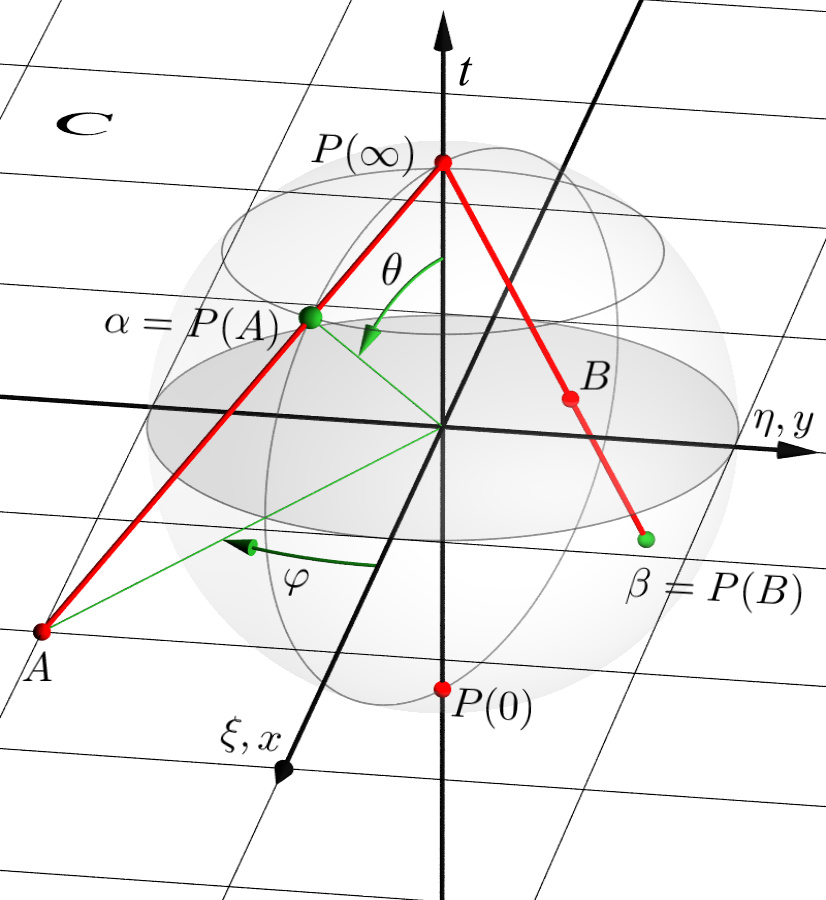
\includegraphics[height=5cm]{07-RiemannSphere}
    \caption{Stereographic projection of a complex number $A$ onto a point $\alpha$ of the Riemann sphere}
\end{figure} 

\begin{theorem}\label{thm:14}
    The set $\mathcal{M}$ of all M\"obius maps on $\mathbb{C}_\infty$ is a group under composition.
    It is a subgroup of $\operatorname{Sym}(\mathbb{C}_\infty)$.
\end{theorem} 

\begin{proof}
    \begin{itemize}
        \item Composition of maps is associative.
        \item $I(z) = z \in \mathcal{M}$ ($a = d = 1, b = c = 0$)
        \item closure:
        \begin{align*}
            \text{Let } f(z) &= \frac{az + b}{cz + d},\ g(z) = \frac{\alpha z + \beta}{\gamma z + \delta} \\
            \text{Suppose } c &\neq 0,\ \delta \neq 0 \\
            \text{First suppose } z &\in \mathbb{C} \setminus \{ - \delta / \gamma \} \\
            \text{Then } f(g(z)) &=  \frac{a \left( \frac{\alpha z + \beta}{\gamma z + \delta} \right) + b}{c \left( \frac{\alpha z + \beta}{\gamma z + \delta} \right) + d} \\
            &= \frac{(a \alpha + b \gamma) z + (a \beta + b \delta)}{(c \alpha + d \gamma)z + (c \beta + \delta d)} \\
            &\in \mathcal{M}
            \intertext{since $(a \alpha + b \gamma)(c \beta + \delta d) - (a \beta + b \delta)(c \alpha + d \gamma) = (ad - bc)(\alpha \delta - \beta \gamma) \neq 0$}
            \text{Also, } f\left(g\left(-\frac{\delta}{\gamma}\right)\right) &= f(\infty) = \frac{a}{c} \\
            \text{and } \frac{(a \alpha + b \gamma) \left(-\frac{\delta}{\gamma}\right) + (a \beta + b \delta)}{(c \alpha + d \gamma)\left(-\frac{\delta}{\gamma}\right) + (c \beta + \delta d)} &= \frac{a \alpha \left(-\frac{\delta}{\gamma}\right) + \alpha \beta}{c \alpha \left(-\frac{\delta}{\gamma}\right) + c \beta} \\
            &= \frac{a}{c} \ \checkmark \\
            \text{Need to check } c &= 0
        \end{align*} 
        \item Inverses: 
        \begin{align*}
            f(z) &= \frac{az + b}{cz + d},\ ad - bc \neq 0 \\
            \text{Let } f^*(z) &= \frac{dz - b}{-cz + a} \\
            \text{Then } f(f^*(z)) &= z = f^*(f(z)) \text{ for } z \neq -\frac{d}{c}, -\frac{a}{c}, \infty 
            \intertext{These cases are ok.}
            \text{If } c &= 0 \\
            f(f^*(\infty)) &= f(\infty) = \infty = f^*(f(\infty)).
        \end{align*}
    \end{itemize} 
\end{proof} 

\begin{theorem}\label{thm:15}
    $\operatorname{GL}_2(\mathbb{C}) / Z \cong \mathcal{M}$ where $Z = \left\{ \begin{pmatrix}\lambda & 0 \\0 & \lambda\end{pmatrix} : \lambda \in \mathbb{C} \setminus \{0\} \right\}$ ($Z$ is the centre of $\operatorname{GL}_2(\mathbb{C})$).
\end{theorem} 

\begin{proof}
    We construct a surjective homomorphism from $\operatorname{GL}_2(\mathbb{C})$ onto $\mathcal{M}$ with kernel $Z$.
    \begin{align*}
        \text{Let } \Phi : \operatorname{GL}_2(\mathbb{C}) &\to \mathcal{M} \\
        \begin{pmatrix}a & b \\c & d\end{pmatrix} &\mapsto f(z) = \frac{az + b}{cz + d}
        \intertext{Note $\Phi$ is a homomorphism}
        f(z) &= \frac{az + b}{cz + d},\ g(z) = \frac{\alpha z + \beta}{\gamma z + \delta} \\
        \Phi \left( \begin{pmatrix}a & b \\c & d\end{pmatrix} \right) &\Phi \left( \begin{pmatrix}\alpha & \beta \\\gamma & \delta\end{pmatrix} \right) (z) = f \circ g(z) \\
        &= \frac{(a \alpha + b \gamma) z + (a \beta + b \delta)}{(c \alpha + d \gamma)z + (c \beta + \delta d)} \text{ from proof of \Cref{thm:14}} \\
        &= \Phi \left( \begin{pmatrix}a & b \\c & d\end{pmatrix} \begin{pmatrix}\alpha & \beta \\\gamma & \delta\end{pmatrix} \right) (z).
    \end{align*} 
    Clearly $\Phi$ is surjective.
    \begin{align*}
        \begin{pmatrix}a & b \\c & d\end{pmatrix} &\in \ker \Phi \\
        \iff \frac{az + b}{cz + d} &= z \; \forall \; z \in C_\infty \\
        \text{Let } z &= \infty \implies c = 0 \\
        z &= 0 \implies b = 0 \\
        z &= 1 \implies a = d \\
        \implies \ker \Phi &= Z
    \end{align*} 
    Finally apply \nameref{thm:six}.
\end{proof} 

\begin{corollary} \label{cor:7} ~\vspace*{-1.5\baselineskip}
    \begin{align*}
        \frac{\operatorname{SL}_2(\mathbb{C})}{\{ \pm I \}} &= \mathcal{M}.
    \end{align*} 
\end{corollary} 

\begin{proof}
    Restrict $\phi$ to $\operatorname{SL}_2(\mathbb{C})$
    \begin{align*}
        \phi : \operatorname{SL}_2(\mathbb{C}) &\to \mathcal{M} \\
        \begin{pmatrix}a & b \\c & d\end{pmatrix} &\mapsto \frac{az + b}{cz + d}
    \intertext{We require $\phi$ to be surjective:}
        f(z) &= \frac{az + b}{cz + d} \\
        &= \frac{ \frac{a}{\sqrt{ad - bc}} z + \frac{b}{\sqrt{ad - bc}} }{ \frac{c}{\sqrt{ad - bc}} z + \frac{d}{\sqrt{ad - bc}} }.
    \end{align*} 
    And $\ker \phi = \{ \pm I \}$.
\end{proof} 

\begin{proposition} \label{prp:13}
    Every M\"obius map can be written as a composition of maps of the following forms:
    \begin{enumerate}
        \item $z \mapsto az$, $a \neq 0$; represents a dilation or a rotation \label{itm:1-1}
        \item $z \mapsto z + b$; a translation \label{itm:1-2}
        \item $z \mapsto \frac{1}{z}$; inversion. \label{itm:1-3}
    \end{enumerate} 
\end{proposition} 

\begin{proof}
    Let $f(z) = \frac{az + b}{cz + d}$. \\
    \begin{align*}
        \text{If } c&= 0;\ z \mapsto \underbrace{\left(\frac{a}{d} \right) z}_{f_1,\ \Cref{itm:1-1}} \mapsto \underbrace{\left( \frac{a}{d} \right) z + \frac{b}{d}}_{f_2,\ \Cref{itm:1-2}} \\
        f &= f_2 \circ f_1 \\
        \text{If } c &\neq 0 \\
        f(z) &= \frac{az + b}{cz + d} = \frac{\left( \frac{a}{c} \right) z + \left( \frac{b}{c} \right)}{z + \left( \frac{d}{c} \right)} \\
        &= \left( \frac{a}{c} \right) + \frac{\frac{-ad + bc}{c^2}}{z + \frac{d}{c}} \\
        &= A + \frac{B}{z + \frac{d}{c}},\ B \neq 0 \\
        z &\underset{f_1,\ \Cref{itm:1-2}}{\mapsto} z + \frac{d}{c} \\
        &\underset{f_2,\ \Cref{itm:1-3}}{\mapsto} \frac{1}{z + \frac{d}{c}} \\
        &\underset{f_3,\ \Cref{itm:1-1}}{\mapsto} \frac{B}{z + \frac{d}{c}} \\
        &\underset{f_4,\ \Cref{itm:1-2}}{\mapsto} A + \frac{B}{z + \frac{d}{c}} \\
        f &= f_4 \circ f_3 \circ f_2 \circ f_1
    \end{align*} 
\end{proof} 

\begin{definition}[Triply transitive action] \label{def:22}
    A group $G$ acts \emph{triply transitively} on a set $X$ if given $x_1, x_2, x_3 \in X$ all distinct and $y_1, y_2, y_3 \in X$ all distinct there exists $g \in G$ such that $g(x_i) = y_i,\ i = 1, 2, 3$. \\
    A group $G$ acts \emph{sharply triply transitively} if such a $g$ is unique.
\end{definition} 

\begin{theorem} \label{thm:16}
    The action of $\mathcal{M}$ on $\mathbb{C}_\infty$ is sharply triply transitive.
\end{theorem} 

\begin{proof}
    Label first triple $\{z_0, z_1, z_\infty\}$ and second triple $\{w_0, w_1, w_\infty\}$.
    We construct $g \in \mathcal{M}$ s.t.
    \begin{align*}
        g : z_0 &\mapsto 0 \\
        z_1 &\mapsto 1 \\
        z_\infty &\mapsto \infty.
    \intertext{First suppose $z_0, z_1, z_\infty \neq \infty$}
        g(z) &= \frac{(z - z_0) (z_1 - z_\infty)}{(z - z_\infty) (z_1 - z_0)} \\
        \text{Check: } ``ad - bc" &= (z_0 - z_\infty)(z_1 - z_\infty)(z_1 - z_0) \neq 0.
    \intertext{If $z_\infty = \infty$}
        g(z) &= \frac{(z - z_0)}{(z_1 - z_0)}
    \intertext{If $z_1 = \infty$}
        g(z) &= \frac{(z - z_0)}{(z - z_\infty)}
    \intertext{If $z_0 = \infty$}
        g(z) &= \frac{(z_1 - z_\infty)}{(z - z_\infty)}
    \intertext{Similarly find $h$ s.t.}
    g : w_0 &\mapsto 0 \\
        w_1 &\mapsto 1 \\
        w_\infty &\mapsto \infty. \\
    \text{Then } f = h^{-1} g : z_i &\to w_i
    \end{align*} 
    Now to prove uniqueness.
    \begin{align*}
        \text{Suppose } f' : z_i &\mapsto w_i \\
        \text{Then } f^{-1} \circ f' : z_i &\mapsto z_i
        \intertext{Let $g$ be as above}
        g f^{-1} f' g^{-1} : 0 &\mapsto 0 \implies b = 0 \\
        : 1 &\mapsto 1 \implies a = d \\
        : \infty &\mapsto \infty \implies c = 0 \\
        \implies g f^{-1} f' g^{-1} &= \text{id} \\
        \implies f^{-1} f' &= \text{id} \\
        \implies f &= f'.
    \end{align*} 
    So, the image of just three points determines the map
\end{proof} 

\subsection{Conjugacy classes in \texorpdfstring{$\mathcal{M}$}{ℳ}}
Recall $\Phi : \operatorname{GL}_2(\mathbb{C}) \twoheadrightarrow \mathcal{M}$ from proof of \Cref{thm:15} ($\twoheadrightarrow$ means its a surjective homomorphism).
Suppose $A, B$ are conjugate in $\operatorname{GL}_2(\mathbb{C})$, i.e. $\exists \; P \in \operatorname{GL}_2(\mathbb{C})$ s.t. $PAP^{-1} = B$ then
\begin{align*}
    \Phi(P) \Phi(A) \Phi(P)^{-1} &= \Phi(PAP^{-1}) \\
    &= \Phi(B) \in \mathcal{M}
\end{align*} 
i.e. $\Phi(A)$ and $\Phi(B)$ are conjugate in $\mathcal{M}$.

Use knowledge of conjugacy classes in $\operatorname{GL}_2(\mathbb{C})$.

\begin{theorem} \label{thm:17}
    Any non-identity M\"obius map is conjugate to $f(z) = \nu z$ for some $\nu \neq 0, 1$ or to $f(z) = z + 1$.
\end{theorem} 

\begin{proof} ~
    \begin{enumerate}
        \item
        \begin{align*}
            \begin{pmatrix}\lambda & 0 \\0 & \mu\end{pmatrix} \text{ where } \lambda &\neq \mu,\ \lambda \neq 0 \neq \mu. \\
            \Phi \left( \begin{pmatrix}\lambda & 0 \\0 & \mu\end{pmatrix} \right) &= f,\ f(z) = \frac{\lambda}{\mu} z = \nu z,\ \nu \neq 0, 1.
        \end{align*}
        \item
        \begin{align*}
            \begin{pmatrix}\lambda & 0 \\0 & \mu\end{pmatrix} \text{ where } \lambda &\neq 0 \\
            \Phi \left( \begin{pmatrix}\lambda & 0 \\0 & \lambda \end{pmatrix} \right) &= \text{id}.
        \end{align*}
        \mathitem \begin{align*}
            \begin{pmatrix}\lambda & 1 \\0 & \lambda\end{pmatrix} \text{ where } \lambda &\neq 0 \\
            \Phi \left( \begin{pmatrix}\lambda & 1 \\0 & \lambda \end{pmatrix} \right) &= f,\ f(z) = \frac{\lambda z + 1}{\lambda} = z + \frac{1}{\lambda} \\
            \text{i.e. } f &= \Phi \left( \begin{pmatrix}1 & \frac{1}{\lambda} \\0 & 1\end{pmatrix} \right). \\
            \text{And } \begin{pmatrix}1 & \frac{1}{\lambda} \\0 & 1\end{pmatrix} &\text{ is conjugate to } \begin{pmatrix}1 & 1 \\0 & 1\end{pmatrix} \\ 
            \text{ via } \begin{pmatrix}\lambda & 0 \\ 0 & 1 \end{pmatrix}  \begin{pmatrix}1 & \frac{1}{\lambda} \\0 & 1\end{pmatrix} \begin{pmatrix}\frac{1}{\lambda} & 0 \\ 0 & 1 \end{pmatrix} &= \begin{pmatrix}1 & 1 \\0 & 1\end{pmatrix}.
        \end{align*}
        So $f$ is conjugate to $g$ where $g(z) = z + 1$.
    \end{enumerate} 
\end{proof} 

\begin{corollary} \label{cor:8}
    A non-identity M\"obius map has either 
    \begin{enumerate}
        \item 2 fixed points or
        \item 1 fixed point.
    \end{enumerate} 
\end{corollary} 

\begin{proof}
    Suppose $g f g^{-1} = h$.
    Then $\alpha$ is a fixed point of $f$ (i.e. $f(\alpha) = \alpha$) $\iff$ $g(\alpha)$ is a fixed point of $h$ (i.e. $h(g(\alpha)) = g(\alpha)$).\footnote{$f(\alpha) = \alpha \iff gf(\alpha) = g(\alpha) \iff h(g(\alpha)) = gfg^{-1}(g(\alpha)) = g(\alpha)$ or $g f = h g \implies h(g(\alpha)) = g(\alpha)$ if $f(\alpha) = \alpha$ and conversely $g(f(\alpha)) = h(g(\alpha)) \implies g(f(\alpha)) = g(\alpha)$.} \\
    So number of fixed points of $f = $ number of fixed points of $h$ as $g$ is a bijection.
    By \Cref{thm:17} either, $f$ conjugate to $z \mapsto \nu z$ which has two fixed points: $0, \infty$; or $f$ conjugate to $z \mapsto z + 1$ which has one fixed point: $\infty$.
\end{proof} 

\subsection{Circles in $\mathbb{C}_\infty$}

A Euclidean circle is the set of points in $\mathbb{C}$ given by some equation $|z - z_0| = r,\ r > 0$.
A Euclidean line is the set of points in $\mathbb{C}$ given by some equation $|z - a| = |z - b|,\ a \neq b$.

\begin{definition}[Circle in $\mathbb{C}_\infty$]
    A \emph{circle in $\mathbb{C}_\infty$} is either a Euclidean circle of a set $L \cup \{\infty\}$ where $L$ is a Euclidean line.
    Its general equation is of the form 
    \begin{align}
        Az\bar z + \bar Bz + B\bar z + C = 0, \label{eq:circle}
    \end{align} 
    where $A, C \in \mathbb{R}$ and $|B|^2 > AC$.
\end{definition}

Where $z = \infty$ is a solution iff $A = 0$. \\
$A = 0$: line \\
$C = 0$: goes through the origin.

There is a unique circle passing through any 3 distinct points in $\mathbb{C}_\infty$.

\begin{theorem} \label{thm:18}
    Let $f \in \mathcal{M}$ and $C$ a circle in $\mathbb{C}_\infty$, then $f(C)$ is a circle in $C_\infty$.
\end{theorem} 

\begin{proof}
    By \Cref{prp:13}, just need to consider 
    $f(z) = az,\ z + b \text{ or } \frac{1}{z}.$
    Let $S_{A, B, C}$ be the circle defined by \Cref{eq:circle}.
    \begin{align*}
        f(z) &= az : S_{A, B, C} \mapsto S_{A / a \bar{a}, B / \bar{a}, C} \\
        f(z) &= z + b: S_{A, B, C} \mapsto S_{A, B - Ab, C + A b \bar{b} - \bar{B}b - B \bar{b}} \\
        f(z) &= \frac{1}{z} = w: S_{A, B, C} \mapsto A + B w + \bar{B} \bar{w} + C w \bar{w} = 0 = S_{C, \bar{B}, A}.
    \end{align*} 
\end{proof} 

\begin{example}
    Consider the image of $\mathbb{R} \cup \{\infty\}$ (a circle in $\mathbb{C}_\infty$) under 
    \begin{align*}
        f(z) &= \frac{z - i}{z + i}.
    \end{align*} 
    It is thus a circle in $\mathbb{C}_\infty$ containing $f(0) = -1, f(\infty) = 1, f(1) = -i$ so $f(\mathbb{R} \cup \{\infty\}) = $ unit circle. 
    Furthermore, complimentary components are mapped to complementary components.
    {\centering 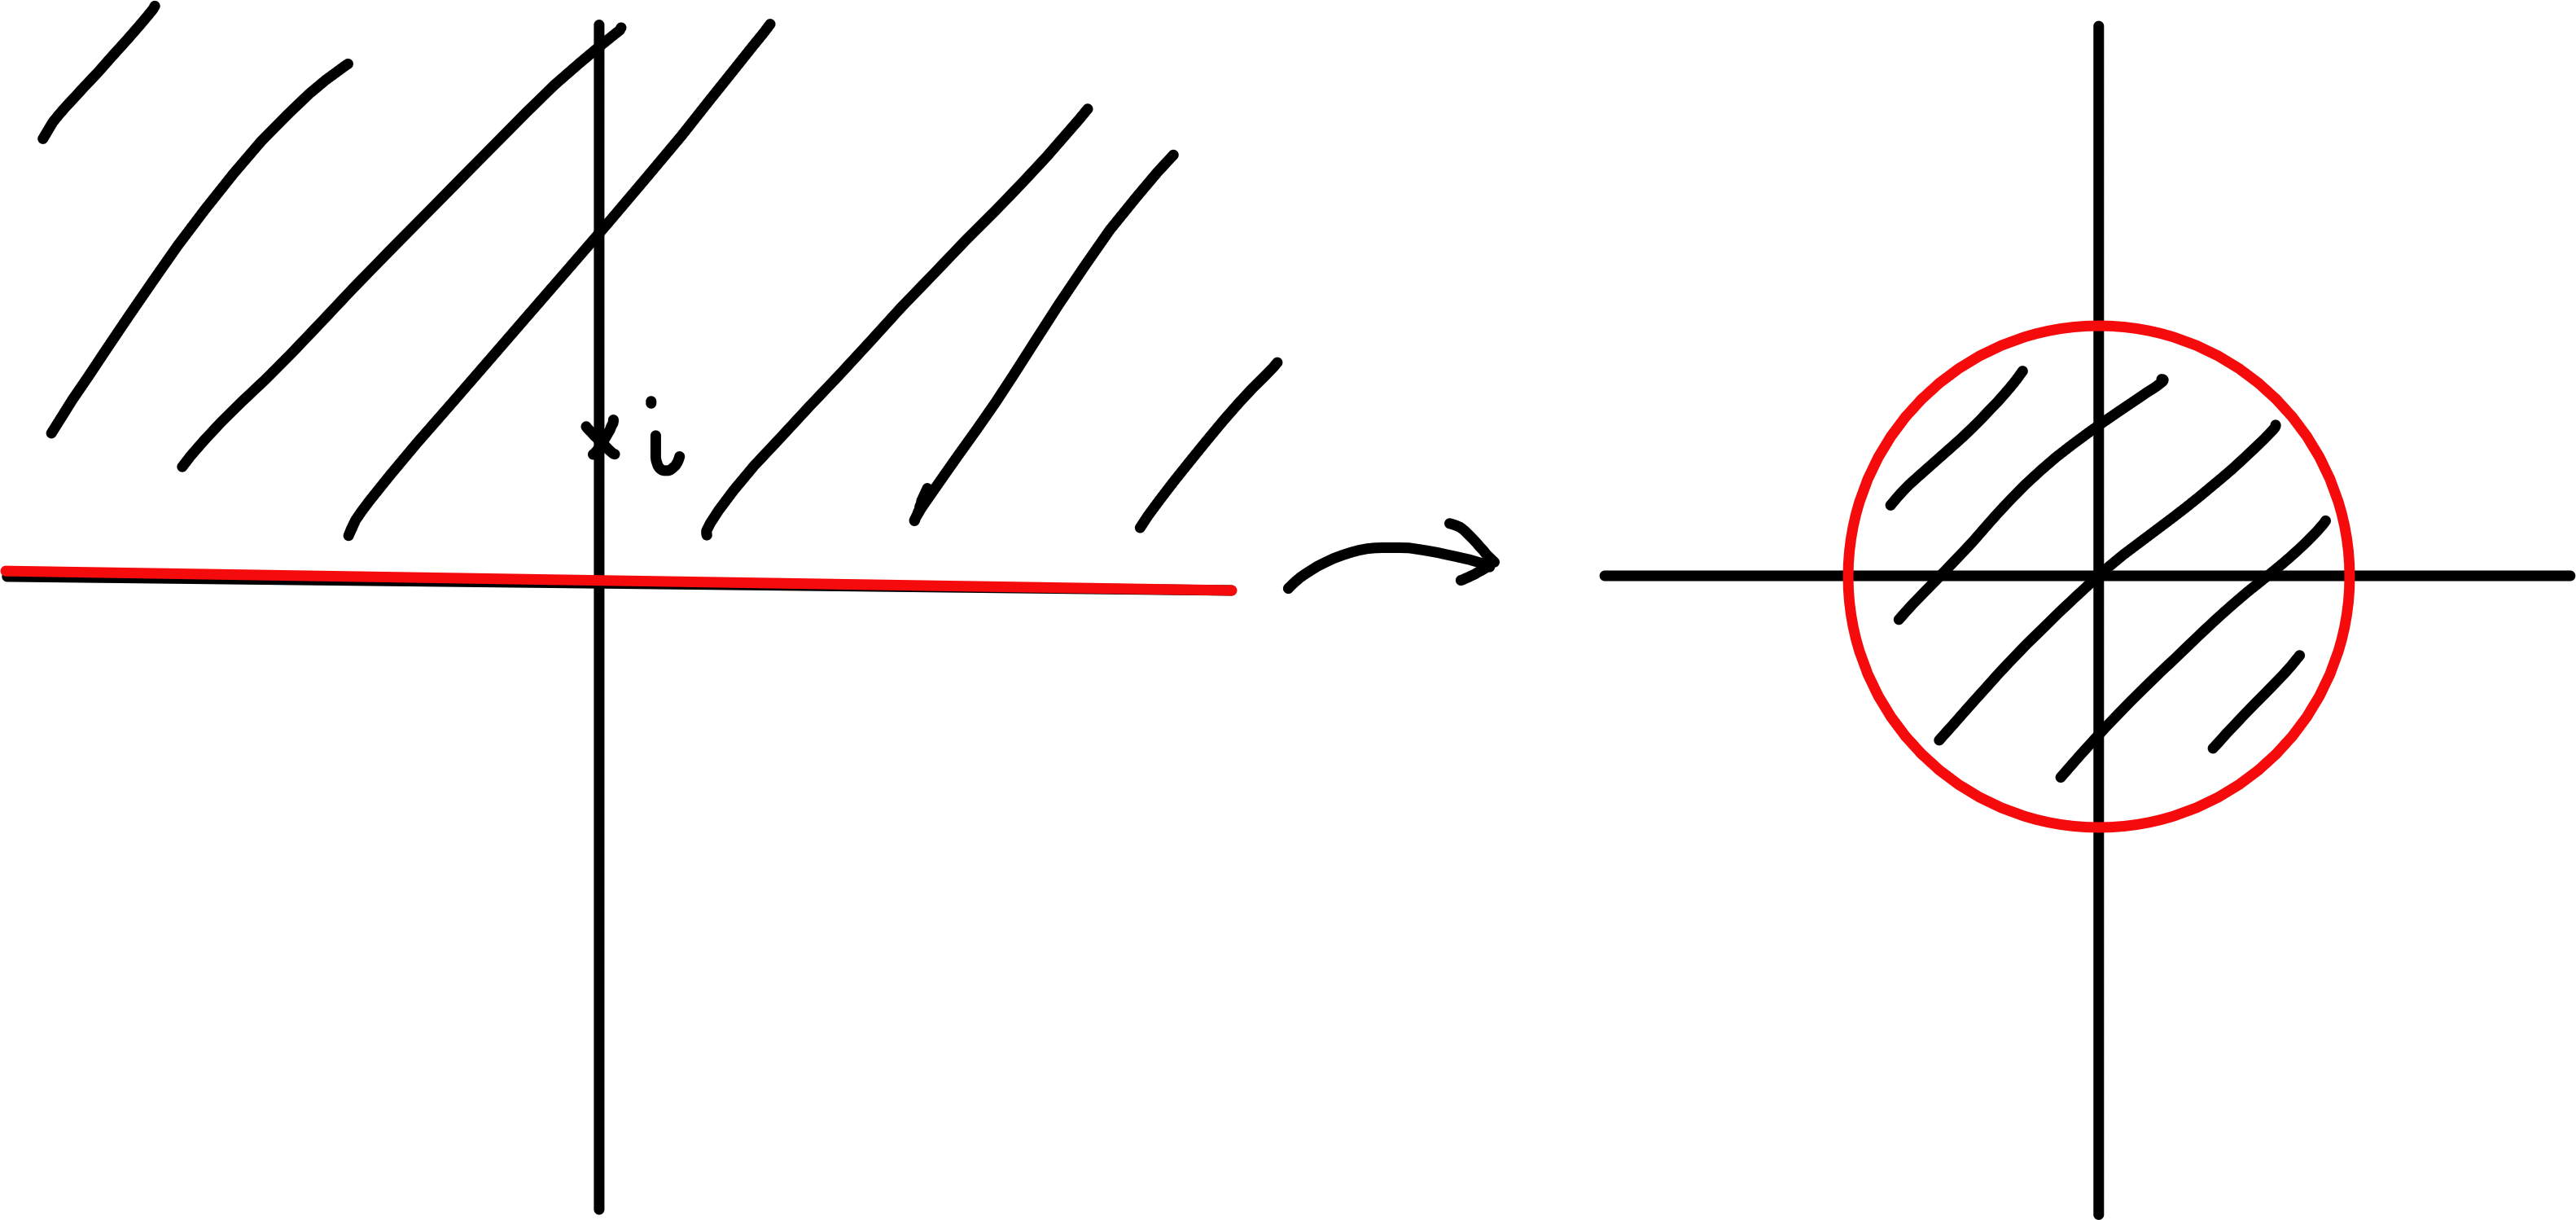
\includegraphics[height=5cm]{08-complimentary}}
\end{example} 

\subsection{Cross-Ratios}

\begin{definition} \label{def:23}
    The cross-ratio of distinct points $z_1, z_2, z_3, z_4 \in \mathbb{C}$.
    \begin{align*}
        [z_1, z_2, z_3, z_4] &= \frac{(z_1 - z_3)(z_2 - z_4)}{(z_1 - z_2)(z_3 - z_4)} \\
        [\infty, z_2, z_3, z_4] &= \frac{(z_2 - z_4)}{(z_3 - z_4)} \\
        [z_1, \infty, z_3, z_4] &= -\frac{(z_1 - z_3)}{(z_3 - z_4)} \\
        [z_1, z_2, \infty, z_4] &= -\frac{(z_2 - z_4)}{(z_1 - z_2)} \\
        [z_1, z_2, z_3, \infty] &= \frac{(z_1 - z_3)}{(z_1 - z_2)} \\
    \end{align*} 
\end{definition} 

Note $[0, 1, w, \infty] = \frac{-w}{-1} = w$

\emph{Warning}: different authors use different permutations of $1, 2, 3, 4$ in the definition.

\begin{theorem} \label{thm:19}
    Given $z_1, z_2, z_3, z_4 \in \mathbb{C}_\infty$ distinct $w_1, w_2, w_3, w_4 \in \mathbb{C}_\infty$ distinct then $\exists \; f \in \mathcal{M}$ s.t. $f(z_i) = w_i \iff [z_1, z_2, z_3, z_4] = [w_1, w_2, w_3, w_4]$.
    In particular, M\"obius maps preserve cross-ratios $[z_1, z_2, z_3, z_4] = [f(z_1), f(z_2), f(z_3), f(z_4)]$
\end{theorem} 

\begin{proof} ~
    ($\implies$): Suppose $f(z_j) = w_j$ and $z_i, w_i \neq \infty \quad \forall \; i$ and $f(z) = \frac{az + b}{cz + d}$, then $cz_j + d \neq 0 \quad \forall \; j$.
    \begin{align*}
        \text{So, } w_j - w_k &= f(z_j) - f(z_k) \\
        &= \frac{(ad - bc) (z_j - z_k)}{(c z_j + d) (c z_k + d)} \\
        \implies [z_1, z_2, z_3, z_4] &= [w_1, w_2, w_3, w_4] \\
        &=  [f(z_1), f(z_2), f(z_3), f(z_4)]
    \end{align*} 
    Need to check other cases; $z_1 = \infty, w_1 = f(\infty) = \frac{a}{c}$ etc.

    ($\Longleftarrow$): Suppose $[z_1, z_2, z_3, z_4] = [w_1, w_2, w_3, w_4]$.
    Let $g \in \mathcal{M}$ s.t. $g(z_1) = 0, g(z_2) = 1, g(z_4) = \infty$ as triple transitive.
    Let $h \in \mathcal{M}$ s.t. $h(w_1) = 0, h(w_2) = 1, h(w_4) = \infty$.
    \begin{align*}
        g(z_3) &= [0, 1, g(z_3), \infty] \\
        &= [g(z_1), g(z_2), g(z_3), g(z_4)] \\
        &= [z_1, z_2, z_3, z_4] \text{ by above} \\
        &= [w_1, w_2, w_3, w_4] \\
        &= [h(w_1), h(w_2), h(w_3), h(w_4)] \\
        &= [0, 1, h(w_3), \infty] \\
        &= h(w_3).
    \end{align*} 
    So $h^{-1}g$ is required map. 
\end{proof} 

So $[z_1, z_2, z_3, z_4] = f(z_3)$ where $f$ is the unique M\"obius map that sends $z_1 \mapsto 0,\ z_2 \mapsto 1,\ z_4 \mapsto \infty$.

\begin{corollary} \label{cor:9}
    $z_1, z_2, z_3, z_4$ lie in some circle in $\mathbb{C}_\infty \iff [z_1, z_2, z_3, z_4] \in \mathbb{R}$.
\end{corollary} 

\begin{proof}
    Let $C$ be a circle through $z_1, z_2, z_4$. \\
    Let $g : C \to \mathbb{R} \cup \{\infty\}$ s.t. $g(z_1) = 0,\ g(z_2) = 1,\ g(z_4) = \infty$.
    \begin{align*}
        g(z_3) &= [0, 1, g(z_3), \infty] \\
        &= [g(z_1), g(z_2), g(z_3), g(z_4)] \\
        &= [z_1, z_2, z_3, z_4] \text{ by \Cref{thm:19}} \\
        \text{So, } [z_1, z_2, z_3, z_4] \in \mathbb{R} &\iff g(z_3) \in \mathbb{R} \\
        &\iff z_3 \in C.
    \end{align*} 
\end{proof} 

\end{document}